%This will basically be a modified form of the FD paper introducing Saphire. Motivate it as a tool for evaluating MD trajectories and predicitng properties.

\noindent\enquote{\itshape He that breaks a thing to find out what it is has left the path of wisdom.}\bigbreak

\hfill Gandalf - The Fellowship of the Ring

\vspace*{0.05\textheight}

In this chapter, we shall present the \texttt{Sapphire} package as published in Faraday Discussions \cite{Sapphy}. We shall motivate the need for this tool, describe the design philosophy, and demonstrate its utility for computing structural, chemical, and photonic properties. This project was a collaborative effort, and where contributions to \texttt{Sapphire} are not the original contribution of the author of this thesis, credit will be duely and appropriately given.

A non-trivial interplay rules the relationship between the structure and the chemophysical properties of a nanoparticle.
In this context, characterization experiments, molecular dynamics simulations and electronic structure calculations may allow to pinpoint the variables that determine a given property.
Conversely, a rigorous computational characterization of the geometry and chemical ordering of metallic nanoparticles and nanoalloys enables to discriminate which descriptors could be linked with their stability and performance.
To this end, we introduce a modular and open-source library, \texttt{Sapphire}, which may  classify the structural characteristics of a given nanoparticle through several structural analysis techniques and order parameters.
A special focus is geared towards using geometrical descriptors to make predictions on a given nanoparticle's catalytic activity.
%
Developing a comprehensive and robust set of taxonomy rules to classify and characterise MNPs and NAs could similarly be beneficial across their large number of multi-disciplinary applications.
%
The objective of this project is to offer the community an open-source and user-friendly package for the structural and chemical analysis of metallic nanoparticles and nanoalloys, released as \texttt{Sapphire}.
%
Whilst there exists software and libraries to characterise structural motifs in molecular and periodic systems \cite{freud2020,oliver_beckstein-proc-scipy-2016,https://doi.org/10.1002/jcc.21787}, we believe that \texttt{Sapphire} fills a gap in the computational chemical physics community by providing an open-source, modular, and documented library dedicated to the computational characterisation of metallic nanoparticles and nanoalloys.

\texttt{Sapphire} is a Python library publicly available at \texttt{https://github.com/kcl-tscm/Sapphire} \cite{Sapphire}, which provides a unified framework to calculate various structural descriptors, from the pair-distance distribution function to the identification of surface atoms. \texttt{Sapphire} extends the common neighbour analysis with the introduction of atomic patterns, allowing a classification into the morphological families, \textit{e.g.,} icosahedra (Ih), decahedra (Dh) and FCC (both with or without stacking fault), as well as amorphous/molten-like motifs. In case of multiple independent simulations and/or long trajectories, \texttt{Sapphire} offers  a robust statistical evaluation  through the use of ensemble averages and well-known statistical quantities, such as the Kullback-Liebler divergence, and statistical tests, like the Kolmogorov-Smirnov test. 

We recommend the use of \texttt{Sapphire} only for metallic nanoparticles and nanoalloys, usually made of at least a chemical species adopting a FCC in the bulk. Although algorithms are independent of the chemistry of the system, the interpretation of results  obtained from Sapphire analysis for periodic structures, and finite-size objects whose components may span the whole the periodic table is far from trivial.

We provide a retrospective overview of \texttt{Sapphire} capabilities. 
Each section presents a didactic introduction to the theory and practical use of each of the characterisation tools. 
Among them, it is worthy to note that \texttt{Sapphire} provides a \texttt{Metadata} section, consistent with the philosophy of the FAIR (Findable, Accessible, Interoperable and Re-usable) principles \cite{https://doi.org/10.48550/arxiv.1805.05039}. 
We thus hope \texttt{Sapphire} will help this community to  more easily create FAIR databases in the future contributions.
%
As paradigmatic examples, we apply \texttt{Sapphire} to characterise individual snapshots as well as molecular dynamics trajectories of Au, Pt, AuPt, CuPt nanoalloys.
%
 
\section{Workflow}
\label{sec:Workflow}

The aim of this section is to briefly discuss \texttt{Sapphire}'s architecture. 
The interested reader is referred to the Github main page, and the tutorial folder in particular, to obtain a complete overview of how Sapphire practically exploits each of its modules.
Indeed, details on how to use the software are available within the tutorial at \texttt{/main/Sapphire/Tutorials/}. 
Furthermore, these web resources will allow the prospective user to reproduce the material in this manuscript with \texttt{Sapphire 1.0.0} given as a free-standing version to accurately reproduce the presented figures.
%

Figure \ref{Sapphire_Workflow}  provides the structure of \texttt{Sapphire} and shows the nature of the decentralised analysis tools. 
%
\texttt{Sapphire} requires as input only the atomic coordinates for the MNP. 
Given that \texttt{Sapphire} leverages the input / output (IO) stream of \texttt{ASE} \cite{ase-paper}, many common formats (\textit{e.g.,} \textit{ .xyz}, \textit{ .exyxyz}, etc...) are compatible. 
%
Note, the coordinate file can be obtained from experimental reconstructions -- e.g., from a tomography experiment -- as well as from numerical simulations. 
As for the nature of the analysis, one may provide a single snapshot, an entire trajectory, or a set of independent trajectories.
%, i.e., as usually occurs using Molecular Dynamics tools. <-- this sentence doesn't make sense:
%sets of independent trajectories do not occur when using molecular dynamics tools
%they are the result of a carefully conceived and statistically meaningfull sampling of the conformation space by means of Molecular Dynamics.
%

\begin{figure}[t!]
    \centering
    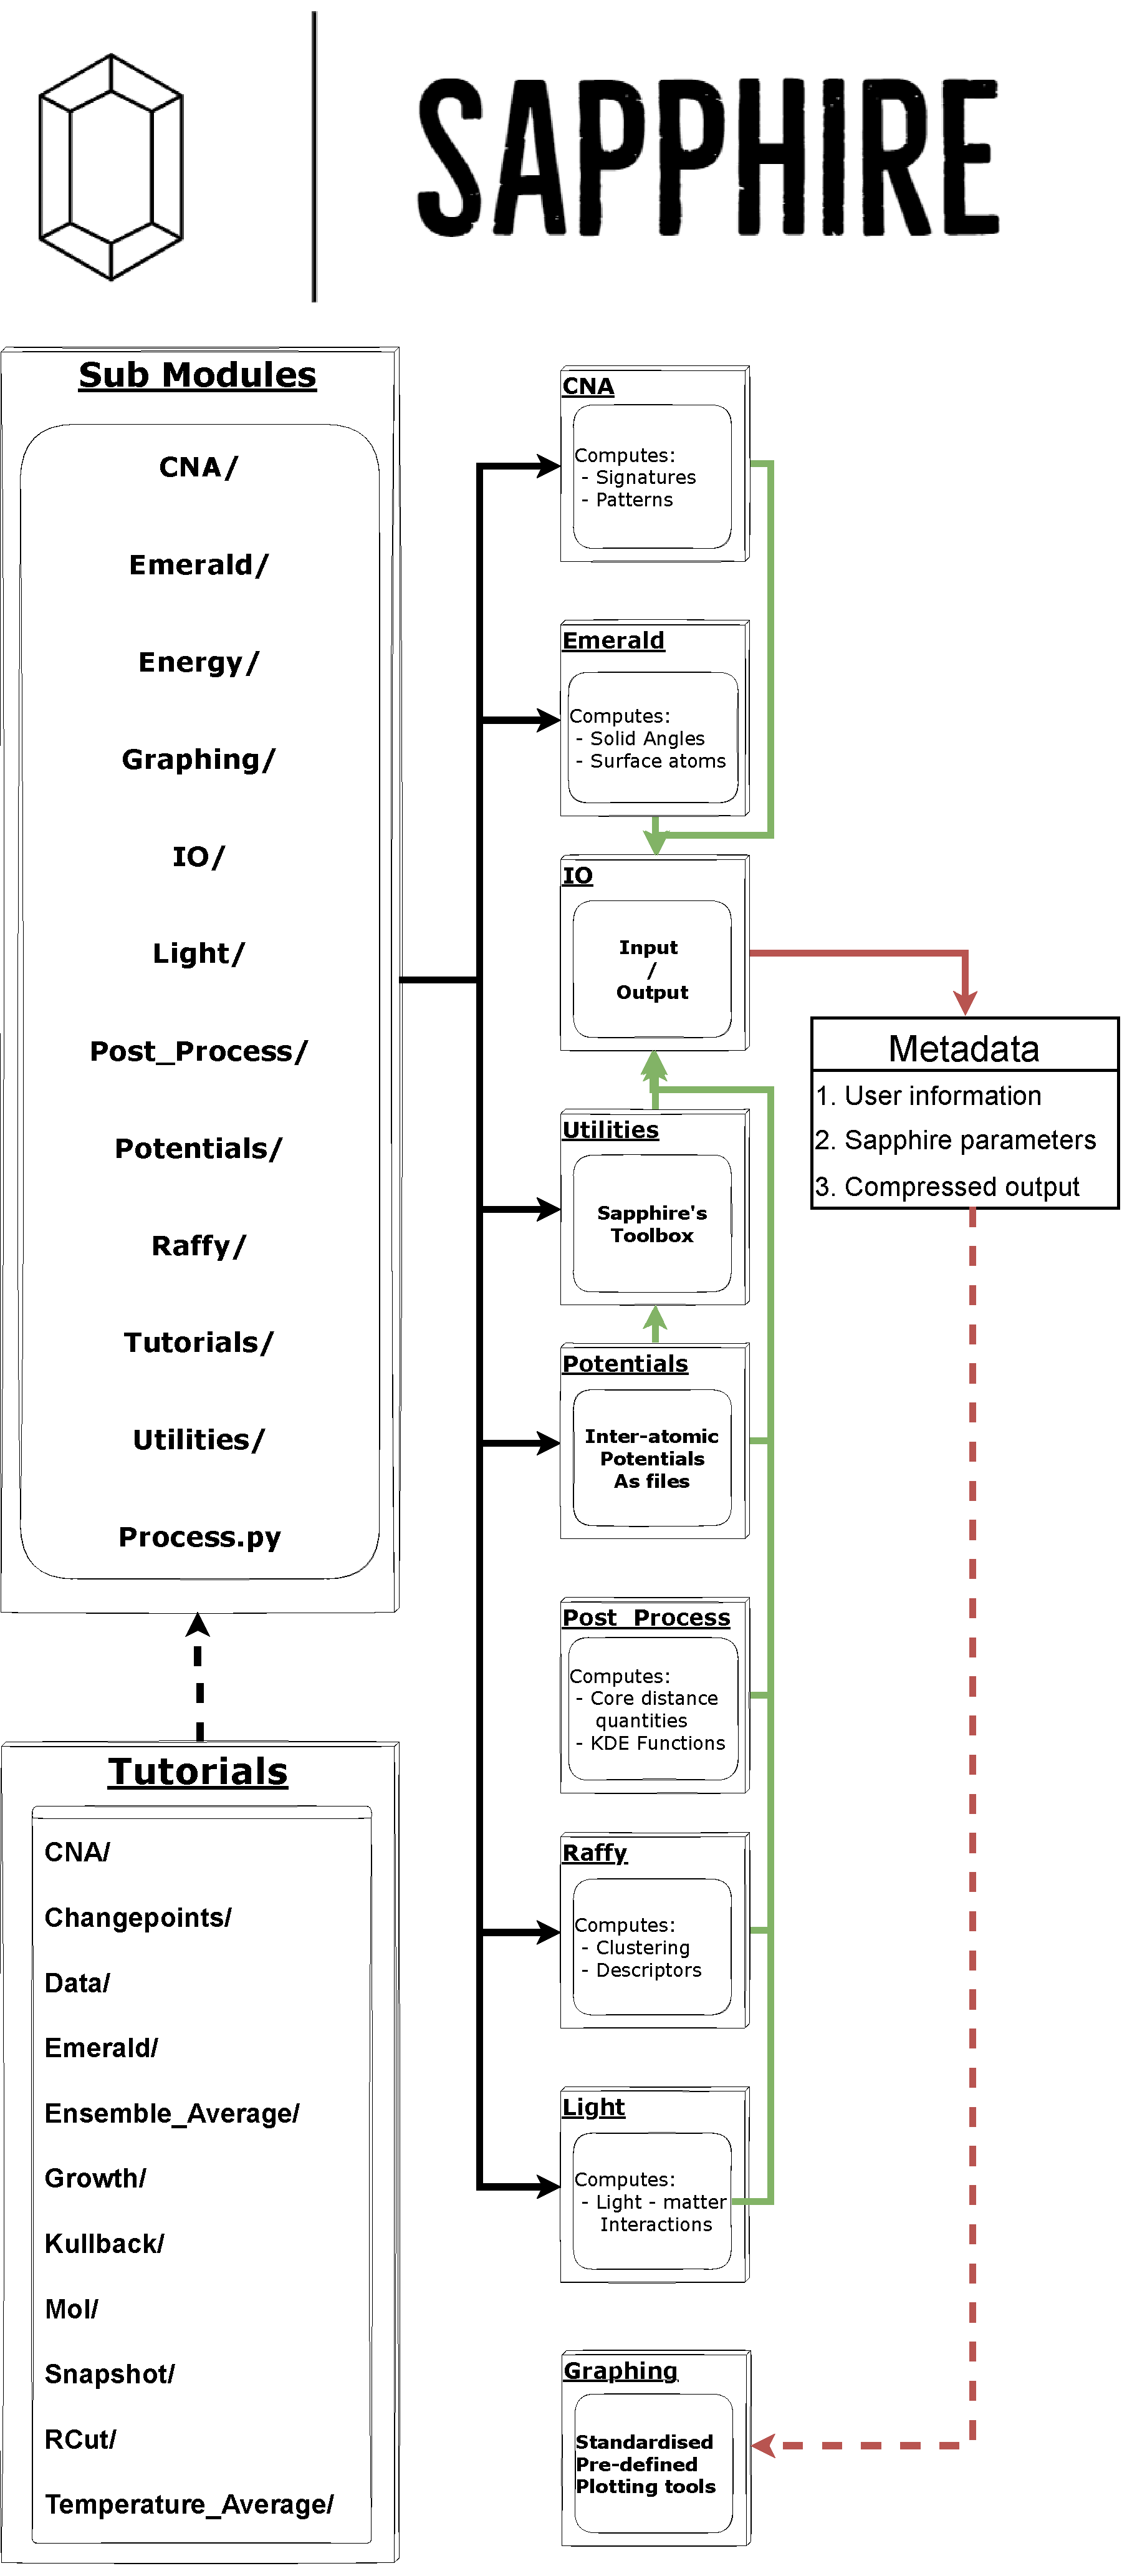
\includegraphics[width=8 cm]{figures/Sapphire/Workflow.pdf}\hfill
\caption{Flowchart detailing the scheme under which \texttt{Sapphire} is executed. Black lines indicate module import directionality. Green lines indicate IO streams, red lines indicate data flow, solid lines indicate hard-coded streams, dashed  lines highlight user choice.}
\label{Sapphire_Workflow}
\end{figure}
%

From here an interconnected nest of sub-modules, organised by common theme, may be accessed. It is worth noting that because the \texttt{Process} class does not directly interact with the IO stream, one may simply call a sub-module to begin the desired analysis.

After gathering the set of configurations to be analysed, \texttt{Sapphire} creates an extended \textit{xyz} file, which encodes user-selected single-atom labels, e.g., its radial distance from the centre of mass, coordination number, and functions thereof. 
Global quantities are both stored in separate files plain text files -- for the Users who like to plot immediately via Gnuplot or the user's plotting tool of choice --  on a  build an architecture for matplotlib, and in the dedicated \texttt{Metadata} object. 
In the following, we describe the quantities, aka descriptors, \texttt{Sapphire} calculates. 
%

A crucial feature of \texttt{Sapphire} is its data storage philosophy. 
Each calculation using Sapphire's \texttt{Process} creates a \texttt{Metadata} in agreement with EMMO \cite{EMMO} and EMMC \cite{EMMC} rules, and the FAIR \cite{https://doi.org/10.48550/arxiv.1805.05039} principles. 
%
\texttt{Sapphire} is amongst the first materials modelling post-processing tools to automatically write metadata in a standardised format, to our knowledge.
%
Contained within the metadata are, among other infos, the following: 
\begin{itemize}
    \item Compressed forms of the written output, to better facilitate a streamlined integration with potential subsequent interactive MNP and NA databases.
    \item User specific information, to enable the community to monitor the provenance of a given data set.
    \item Specifically chosen parameters for post-processing tools (each parameter is described in details in the online manual).
\end{itemize}
%

The final stage of the flowchart in Figure \ref{Sapphire_Workflow} lies in the use of \texttt{Graphing} tools. 
This is a library of pre-prepared \texttt{matplotlib} templates which may be called by the \texttt{Plot\_Funcs} object defined within the library. 
From this, the \texttt{Figures object} is constructed from the collected metadata and the user requested input quantities.
%
This parses the lists of input parameters for each requested plotting function and introduces Sapphire's defaults, should any arguments be omitted. 
%
We then call the \texttt{Make$\_$Plots} function of the Figures object which iterates over all of the plotting functions, passing into each one the relevant list of input arguments.

\section{\texttt{Sapphire} descriptors}
\label{sec:PDDF}

In this section, we list and explain the analysis that \texttt{Sapphire} performs. We first discuss the distance related properties as their are fundamental to introduce a cutoff and hence the concept of local environment for any further analysis.

\subsection{Distance Distribution Functions}
The distribution of pair-atomic distances (pair-distance distribution function, PDDF) is a crucial quantity to characterise the geometry and chemical ordering of an NA. 
Further, the PDDF is a directly measurable quantity via X-ray techniques \cite{Neder_2005,Nederkc5105}.
%

To define the PDDF, let $d_{ij}$ be the pair-distance between atoms $i$ and $j$:
\begin{equation}
    d_{ij} = \sqrt{ (x_{i}-x_{j})^{2} + (y_{i}-y_{j})^{2} + (z_{i}-z_{j})^{2} } \mbox{~~~.} 
\end{equation}
We then calculate the PDDF via a Kernel density estimates (KDE), constructed from $n$ observations:
\begin{equation}
    PDDF\left[K\left(d_{ij},d;h\right)\right] = \frac{1}{Nh} \sum_{i}^{N} \sum_{j\neq i} K\left(\frac{d_{ij}-d}{h}\right)
    \label{eqn:KEDE}
\end{equation}
%
where $K\left(d_{ij},d;h\right)$ labels the kernel function over the $d_{ij}$ variable, and the parameter $h$ is the bandwidth that defines the tightness of the kernel function.
%
Note that the KDE assumes that each interatomic distance has been randomly drawn from a given distribution, which the user may define via input.
The Gaussian distribution is the default choice.
Alternatives, such as the Epanechnikov \cite{epan}, and the uniform distribution, are also currently supported. 

Figure \ref{fig:pddf_params} shows the effect of the $K$ and $h$ choice in the PDDF calculation, as a function of the independent parameter $d$, written in terms of the lattice bulk $a_0$. 
Setting the bandwidth, $h$, is a delicate step. The $h$-choice should balance a too fine resolution ~-~ where each distance might be present a single time, and below any reasonable resolution ~-~ and a too large one ~-~ where different neighbour shells are projected onto the same distance width. 
%We suggest to consider values below half of the distance between the first and second nearest neighbour as the proper choice for distinguishing nearest neighbours peaks in solids.
%
As a default, we have set the bandwidth to be 0.05 of the bulk lattice, which we have found to be sufficiently broad to smooth the sharp Dirac peaks from having a finite sample, and to sufficiently resolve key features, \textit{i.e.,} the first peak, minimum, and the second peak (orange line in Figure \ref{fig:pddf_params}. In principle, one may consider the h parameter to be comparable to the resolution in various microscopy techniques. As such, deviating from the default value must be done whilst considering the physical meaning of this parameter. That is to say that measuring interatomic distances to arbitrary precision is not possible at finite temperatures due to lattice vibrations.
%
\begin{figure}[ht!]
    \centering
    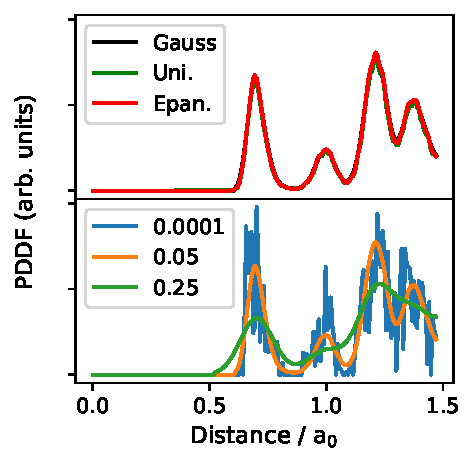
\includegraphics[width=7.5cm]{figures/Sapphire/PDF_Example.pdf}`
    \caption{The three possible parameterisations for calculating the PDDF using Eq. \ref{eqn:KEDE}. Top panel demonstrates the agreement between available kernels where $h=0.05$. Bottom panel illustrates the dependence on the bandwidth, $h$, orange (0.05 a$_{0}$), blue (0.0001 a$_{0}$) and (0.25 a$_0$) green with a$_{0}$ set to be the bulk lattice parameter. We have selected a randomly alloyed AuPt NA of 1415 atoms arranged as an icosahedron with a ratio of Au:Pt of 4:1.}
    \label{fig:pddf_params}
\end{figure}

Given the analytical form of the KDE, derivatives can be easily calculated, and the approximate location of minima (and maxima) in the distribution can be identified. This is a key utility. 
%
The first PDDF minimum is instrumental to a robust determination of nearest neighbour distance. 
The position of the second maximum may also allow to identify whether the NA loses its symmetry or undergoes a structural or phase change. The latter should be associated to an overall radial breathing of the NA. 
%
\begin{figure}[ht!]
    \centering
    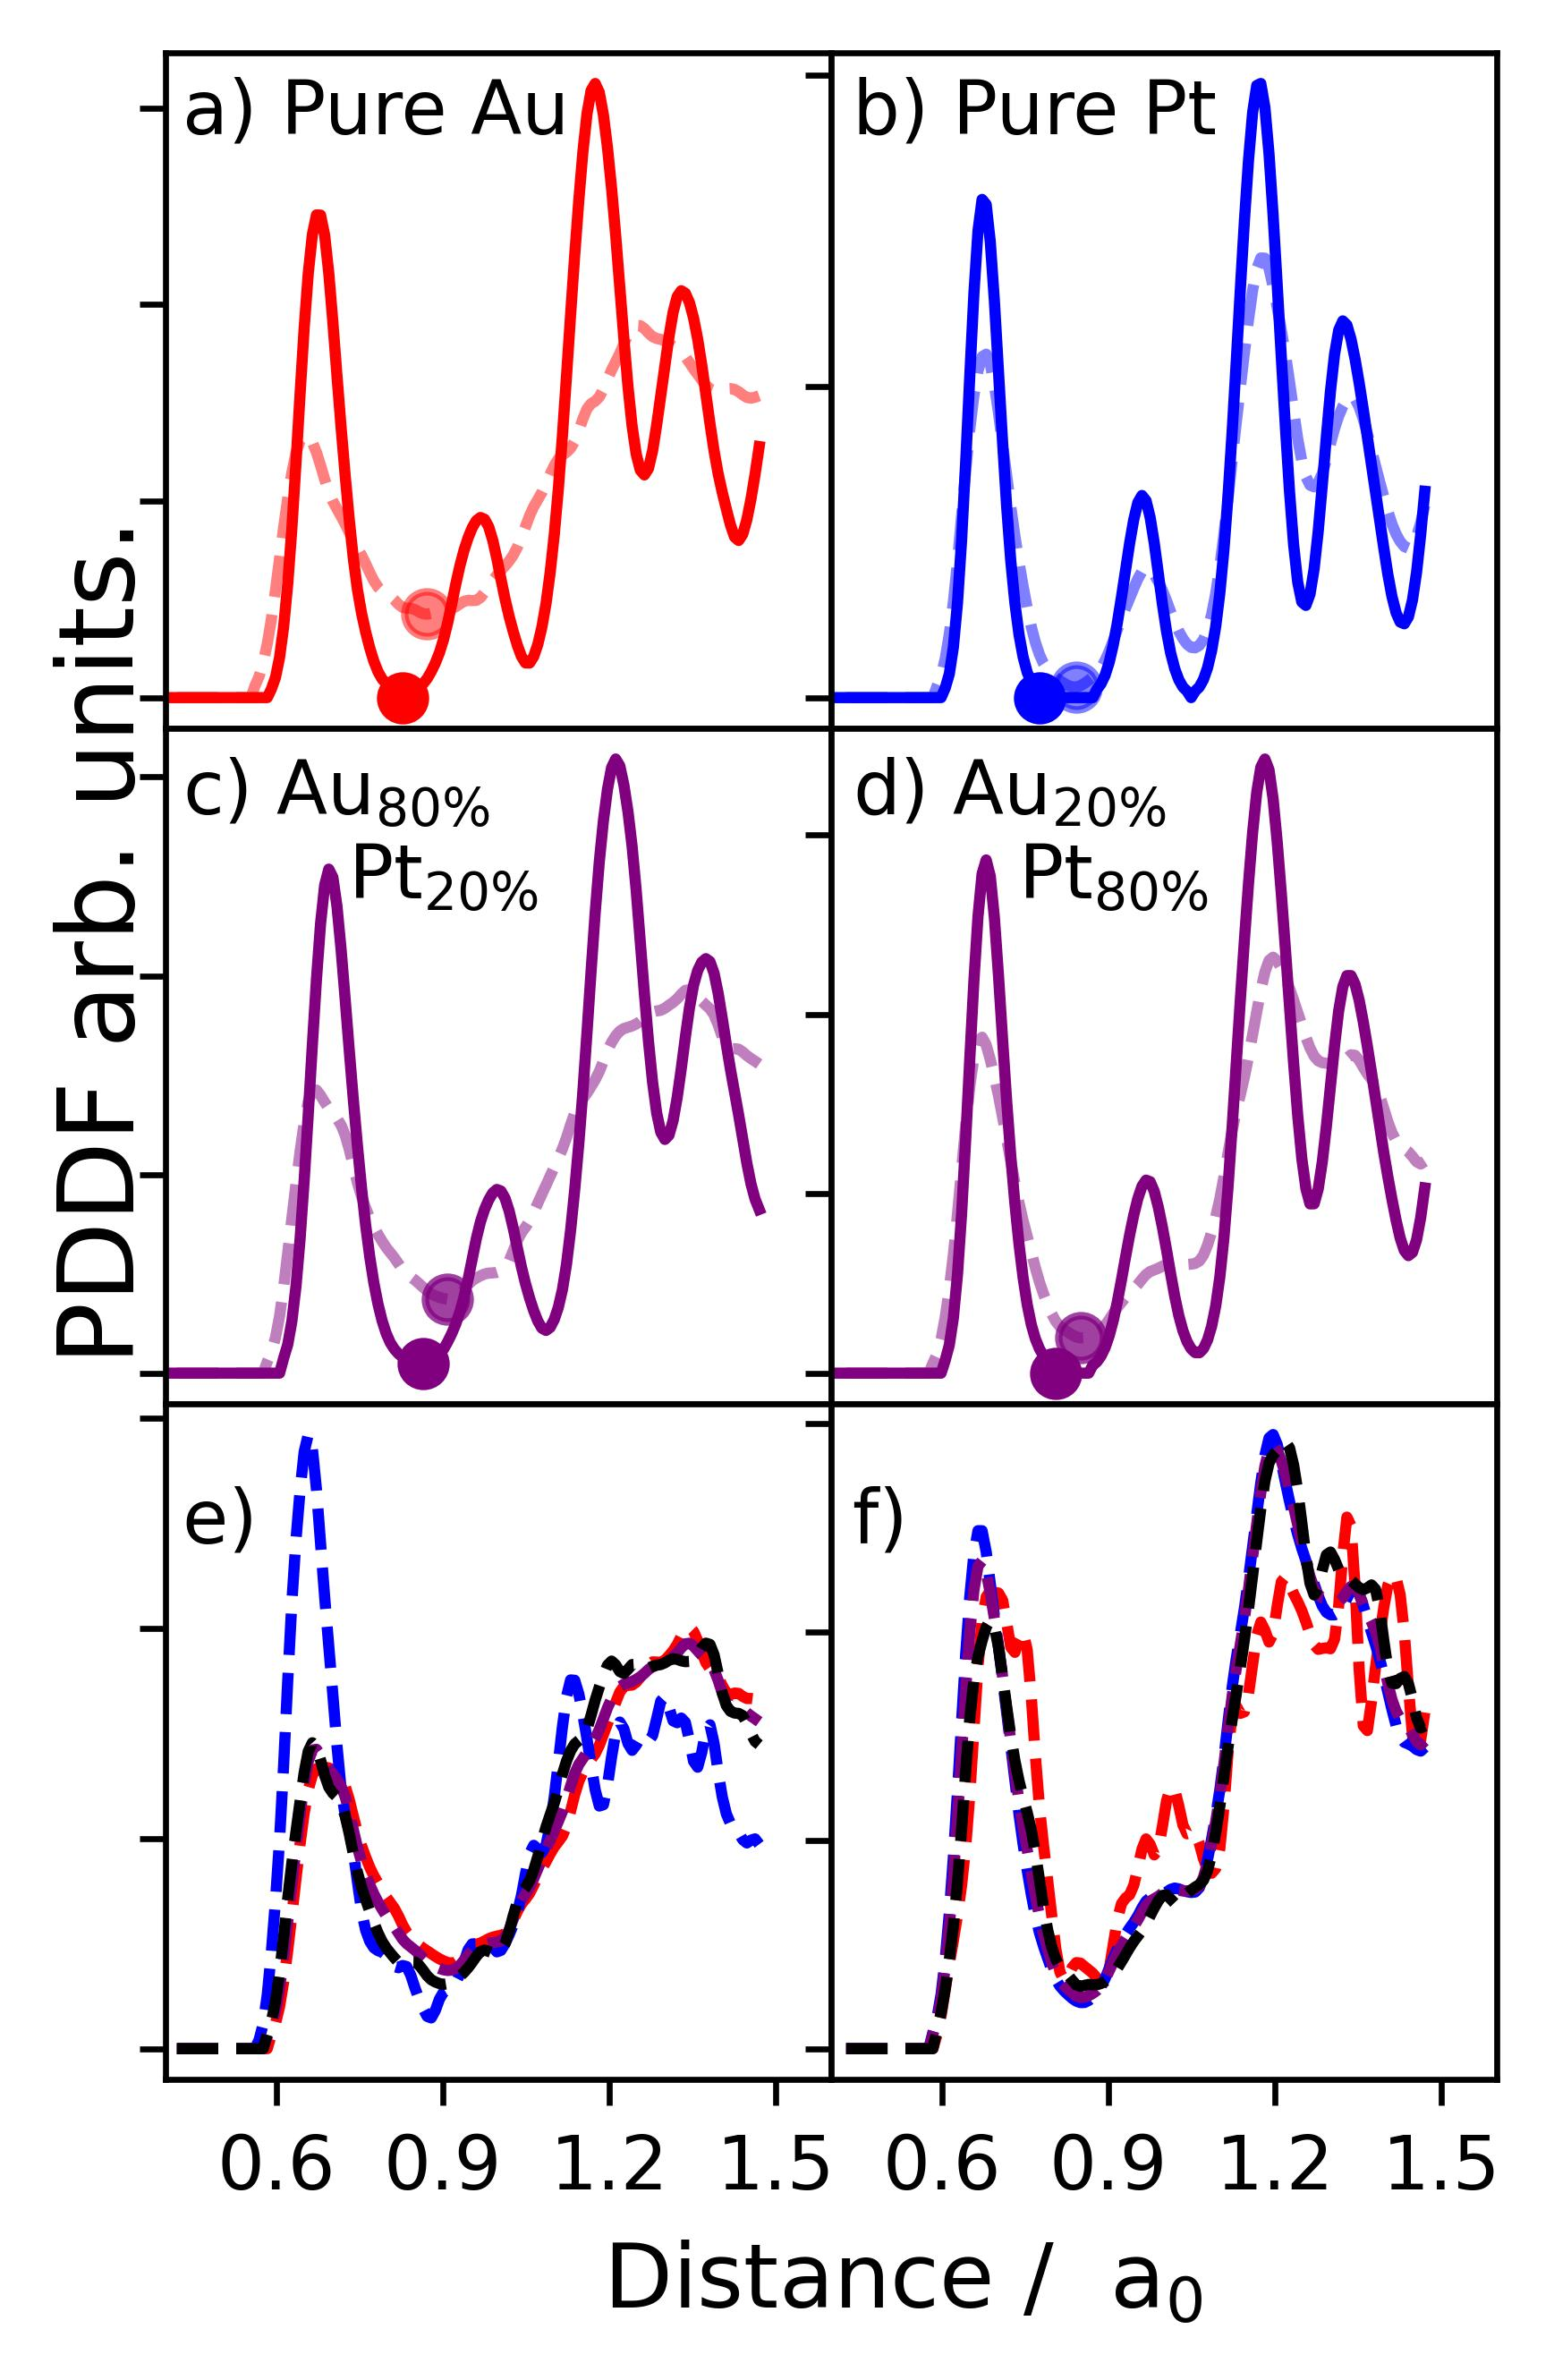
\includegraphics[width=7.5cm]{figures/Sapphire/pddf.jpeg}
    \caption{
    PDDF computed with \texttt{Sapphire} for a set of pure Au, Pt, and AuPt NAs containing 1415 atoms and adopting initially an icosahedral (Ih) shape.
    Distances are scaled with respect to the bulk lattice distance $a_{0}$. For NAs, this measure is taken as the average of the two pure metals' bulk lattice distance. Panels (a) and (b) refer to pure Au and pure Pt MNPs, respectively. Panels (c) and (d) refer to randomly alloyed AuPt NAs at different chemical compositions, as indicated in the inset. Solid lines correspond to the PDDF sampled at 300 K while dashed lines are taken at 1000 K. Dots represent the position of the first PDDF minimum, corresponding to $R_{cut}$. Panels \textbf{e)}, \textbf{f)}, \textbf{g)}, and \textbf{h)} present the PDDF for homo interactions (Au - red, Pt - blue, Cu - green), and hetero interactions (black).}
    \label{fig:pddf}
\end{figure}

The evolution of the pair-distance distribution function (PDDF), independently of their chemical label, enables the:
\begin{itemize}
    \item Identification of a cut-off distance ($R_{cut}$) set as where the first minimum in the PDDF falls. Such definition of  radial distance allows the subsequent definition of a local environment, and the construction of the adjacency matrix.
    \item Detection of solid, liquid, and amorphous, depending on the position of the second peak of the PDDF. A robust definition of "amorphous/ molten-like" shape is where there is not a maximum in correspondence of the bulk lattice, $a_0$, and the maximum radial distance is comparable with other well ordered shapes. The same future and a radial breathing refers to a solid to liquid transition \cite{Delgado-Callico2021}.
\end{itemize}
%

To clarify further this points, Figure \ref{fig:pddf} details the PDDFs of pure MNP with 1415 atoms of Au, Pt, and AuPt with two different compositions. The reported simulations data are obtained from iterative molecular dynamics runs, as available in \texttt{LoDiS} \cite{Pavan2018,Rossi2018,LoDiS}, where the temperature is increased by 50 K each 1 ns, from 300 K to 1000 K.
%

We show PDDF sampled at both cold (solid lines in panel (a)-(d) Figure \ref{fig:pddf}) or high temperatures (dashed lines in the same panels). 
We note a broadening of the first peak at higher T, for both pure and alloyed nanosystems. At the same time, it is evident that the position of the first peak does not change significantly with the temperature. 
%
We stress that a radial cut-off can be defined independently of the temperature, as highlighted by the full-circle dots marking the position of the first minimum \cite{Delgado-Callico2021,Zeni2021}.
The position of the second peak instead clearly changes between cold and hot temperatures. 
This is particularly evident in the case of pure Au and Au-based nanoalloys. 
Pt-NAs just show a minor effect because they are still approaching their melting point. Indeed, the pure Pt-NP PDDF still presents a clear peak in correspondence of its bulk lattice distance. 
For NAs with a large amount of Pt, the second peak also still presents a shoulder in correspondence of the bulk lattice, suggesting that the phase change starts mainly in the gold network (see panel (f) of Figure \ref{fig:pddf} PDDF-line corresponding to Au-Au and Au-Pt bonding). 

\texttt{Sapphire} also supports the pair correlation function, $g(r)$, as used to describe long-range order in liquids \cite{10.1039/9781847558237} and is related to the structure factor.
%
\begin{equation}
    g\left( r \right) = \frac{ dn\left( r \right) }{ 4\pi r^{2}\rho dr } \mbox{~~~,}
    \label{eqn:gofr}
\end{equation}
%
where $\rho$ is the bulk density of atoms, $dn(r)$ is the number of atoms within the spherical shell of thickness of $dr$.


The 3D chemical ordering of a nanoalloy can be qualitatively, if not quantitatively, extracted from the radial distribution function (RDF) of the chemical species in the NA. %
Similarly to the PDDF, this density quantity can be readily extracted from both numerical simulations and (line-scan) experiment \cite{Neder_2005}.
%
To this goal, \texttt{Sapphire} provides three complementary radial distributions as we can identify possible atomic interaction environments: the whole system, labelled with a $w$, the sub-regions -or sub-clusters- A and B which gather only atoms A and B, respectively. \texttt{Sapphire} calculates (i) the density of atoms, independently of their chemical species, from the centre of mass of the whole NA, $CoM_w$; (ii) the distribution of atoms-A from their centre of mass, $CoM_A$; and (iii) similarly for B-atoms, from the $CoM_B$. 
%
The RDFs count the number of atoms falling in concentric shells from the centre of mass of the nanoparticle:
\begin{equation}
    r_{\alpha}(i \in w, A, B) = \sqrt{\hat{x(i)}_{\alpha}^2 + \hat{y(i)}_{\alpha}^2 + \hat{z(i)}_{\alpha}^2}
\end{equation}
where the coordinates $\hat{x}_{\alpha},\hat{y}_{\alpha},\hat{z}_{\alpha}$ of the atom-$i$ and chemical species $\alpha = A,B$ are re-scaled w.r.t the centre of mass chosen, namely whole NA, or A, and B sub-regions.
%
As was the case for computing the PDDF, we may also apply the KDE approach to compute the RDFs for each of the three types of radial distribution described above:
%
\begin{equation}
    RDF\left[K\left(d_{ij \in w, A, B},d;h\right)\right] = \frac{1}{Nh} \sum_{i}^{N} \sum_{j\neq i} K\left( dist (CoM_{w, A, B}) \right)
    \label{eqn:rdf}
\end{equation}
%
In principle, Eq. \ref{eqn:rdf} can be extended to more than two chemical species, where we consider all the independent sub-regions occupied by each element.
%

For binary nanoalloys, behind the how atoms are radially distributed, a handy and easy quantity to characterise the chemical ordering is the relative distance of the centre of mass of the two chemical sub-regions, $\Delta(CoM)$. This quantity is a easy and robust descriptor to monitor the formation and the evolution to/from Janus and quasi-Janus chemical orderings \cite{D2CP00648K},
\begin{equation}
    \Delta(CoM) = \sum_{i \in A} \frac{r_{i,A}}{N_A} - \sum_{i \in B} \frac{r_{i,B}}{N_B} 
\end{equation}
where $r_{i,A \in A}$ is the radial distance of the atom-$i$ of species A taken from the centre of mass of the nanoparticle. Similarly, for the B sub-cluster. $N_A(B)$ is the number of atoms A(B) in the nanoparticle. $\Delta(CoM)$ is expected to be close to zero for alloyed, core-shell, and multi-shell ordering, but not zero when the phase-segregation breaks the radial symmetry. We provide in Figure \ref{fig:ens-avg} an example of this measure, averaged over independent ensembles. 

\subsection{Adjacency matrix based descriptors}

The definition and characterisation of nearest neighbour networks has been largely adopted to classify nanoparticle and nanoalloy morphology and draw structure-property relationships \cite{C8NR02278J,Perea2015,Stukowski_2012}.
%

To evaluate nearest neighbour networks and quantities deriving from the latter, solely according to a distance criterion, the adjacency matrix \textbf{A} is defined as:
\begin{equation}
        \textbf{A} \left( r_{ij} \right) = \begin{cases}
    1 ,& \text{if } r_{ij}\leq R_{cut}\\
    0,              & \text{if } r_{ij} > R_{cut}
\end{cases} 
    \label{eqn:CN}
\end{equation}


One of the first quantity mentioned in any solid state books is the number of neighbours for the various Bravais lattice. 
With a focus on catalysis, the coordination of an adsorption site has been often used as a descriptor to rationalise its activity. 
Still related to the ability of a system to bind other molecules, in biophysics and soft matter, several algorithms have been developed to estimate the number of nearest neighbours of a macromolecule \cite{vanmeel2012}
%
A simple chemical intuition suggests that low-coordinated atoms are more likely to form chemical bonds than highly-coordinated ones.
%
The coordination number of an atom $j$, $CN_{j}$,   follows from the adjacency matrix:
\begin{equation}
    CN_{j} = \sum _{i \neq j} \textbf{A} \left( r_{ij} \right) \mbox{~~~.}
    \label{eqn:CN_VM}
\end{equation}
Nonetheless, this definition might suffer of finding a suitable cut-off that might not be always easy to select, especially for nanoalloys with a large mismatch.

The definition of more complex local atomic environment descriptors may be written as a function of the coordination number. \texttt{Sapphire} calculates two descriptors, namely the atop generalised coordination number (aGCN) and the mixing parameter $\mu$. 

The atop generalised coordination number (aGCN) \cite{Calle-Vallejo2014} is defined by equation \ref{eqn:aGCN}
with $CN_{max}$ set to 12, as this is the coordination of an FCC atom in the bulk. we point out that for metallic systems, it seems reasonable to consider the total coordination of each atom $j$ regardless the difference in electronegativity of the chemical species.
%
The reason why we suggest to look at the aGCN is three-fold. First, it has been shown to provide a robust linear relationship with the adsorption energy of small molecules (e.g., O, CO, OH) \cite{Calle2015}.
Second, the aGCN is able to characterise the nanoparticle's surface sites - avoiding the basic classification into face, edge, vertex -- and to classify a nanoparticle geometry on the basis of its aGCN-genome \cite{Rossi2019}.
%
Finally, the use of the aGCN offers a route to estimate the surface area, beyond, e.g., spherical approximations. 
%
The nanoparticle's surface can be well approximated by writing it as a sum over atomic contributions, which are a function of the atomic radius $r_{at}$ weighted with their aGCN. The latter is a measure of how much they are "exposed": \cite{Rossi2020}

A full comparison of the surface area calculated for closed shell geometries using cluster spherical approximation, geometrical consideration, and based on the aGCN has been reported in Ref. \cite{Rossi2020}.

\begin{figure}[t!]
    \centering
    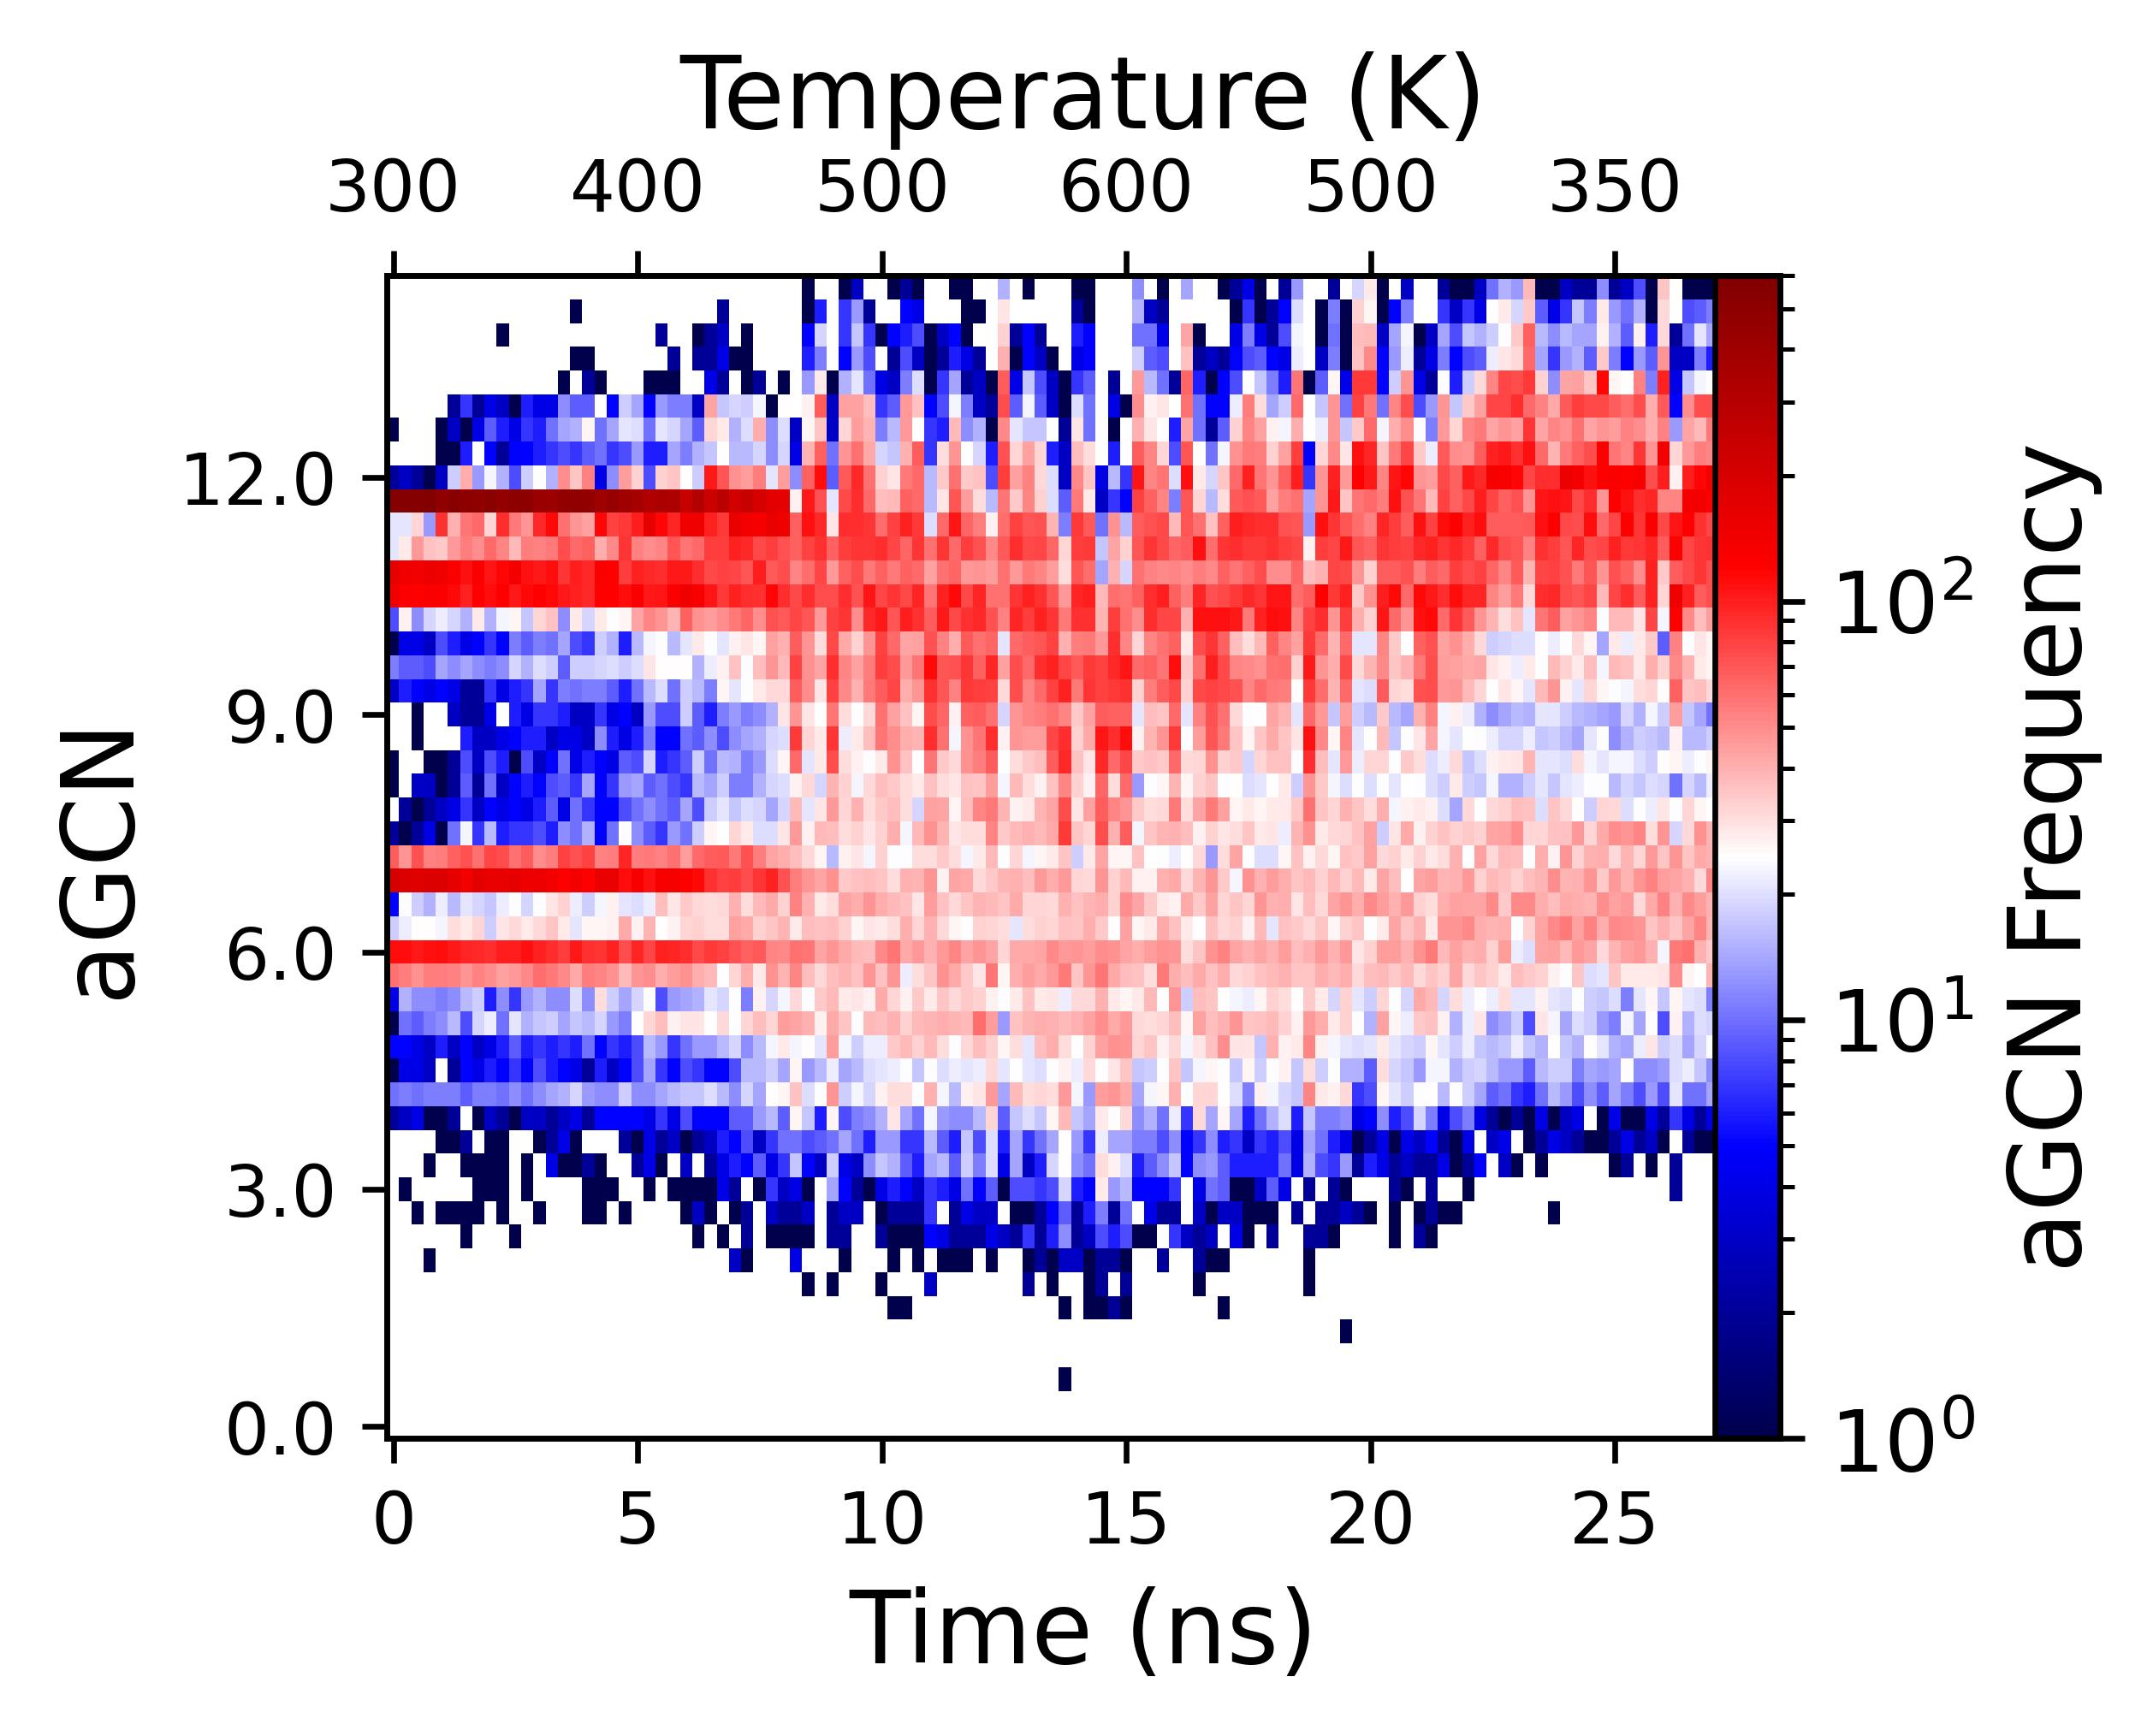
\includegraphics[width = 8cm]{figures/Sapphire/aGCN.jpeg}
    \caption{Heat-maps demonstrating the evolution of the aGCN distribution, as calculated via the adjacency matrix, with respect to time for two types of dynamical processes. Panel \textbf{a)}: two Pt$_{55}^{Ih}$ NAs deposited atop an Au$_{2057}^{Ih}$ MNP maintained at 600 K for 100 ns. Panel \textbf{b)}: randomly alloyed Au$_{1283}$Pt$_{132}$ NAs with the initial morphology of an Ih heated from 300 K (t=0) to 1000 K t=12 ns) and then cooled back to 300 K (t=24 ns). }
\label{fig:agcn}
\end{figure}

We show in Figure \ref{fig:agcn} the evolution of the distribution of the aGCN for the specified nanoalloy. Recall that the assumption of a maximal number of neighbours in the bulk phase is 12, in accordance with a well-ordered FCC-like environment. However, here we demonstrate that larger values may indeed be reported for highly disordered structures. Further confounding this is that the aGCN is a function of the adjacency matrix, which itself depends on a pre-determined cutoff radius which may dynamic with respect to time due to the high mobility of atoms at finite temperature and possible thermal dilation effects. Moreover, one may consider the model described in Section \ref{sec:electrocat}. With an appropriate choice of model parameters, it is both simple and efficient to use this aGCN distribution to make predictions regarding the time dependent electro-catalytic efficacy of a given nanoalloy.

In the case of nanoalloys, we can easily separate the local environment of each atom between homo-pairs and hetero-pairs. 
Counting the A-A, $NB_{AA}$, B-B $NB_{BB}$, and A-B pairs, $NB_{AB}$ enables to evaluate the mixing parameter $\mu$.
The latter is a useful parameter for a fast characterisation of the NAs chemical ordering :
\begin{equation}
\mu = \frac{NB_{AA} + NB_{BB} - NB_{AB}}{NB_{AA} + NB_{BB} + NB_{AB}} {\mbox ~~~,}
\end{equation}
where $\mu$ tends to -1 when the NA is fully alloyed, and to +1 when there is a complete phase separation.

\subsection{Concertedness and collectivity of a morphology rearrangement}

Monitoring time-dependent changes in the adjacency matrix, over successive time-steps, allows to characterize whether structural rearrangements took place, and if these involve concerted and/or collective rearrangements.
%
In this context, we adopt the definitions first put forward in Ref. \cite{Rossi2018}.

Let $AA_{ij}(\Delta t)$ be
a matrix counting the absolute number of bonds formed or lost between each $ij$ pair of atoms, within a characteristic time length $\Delta t$:
\begin{equation}
    AA_{ij} \left( \Delta t \right) = \vert A_{ij} \left( t + \Delta t \right) - A_{ij}(t) \vert
\end{equation}
%$AA_{ij}$ is then equal to 0 if no bonds are broken/formed.
From this quantity, the system mobility, $R(t, t + \Delta t)$, is measured by summing over single atom mobility:
\begin{eqnarray}
 \nonumber   R(t, t +\Delta t) =\sum_i R_i(t, t +\Delta t)
\\
R_i(t, t + \Delta t) = \sum_{j\ne i} AA_{ij} (\Delta t)
\end{eqnarray}
%
To measure the collectivity of a mechanism, $H$, one then counts the ratio of atoms which change at least one neighbour within a  $\Delta t$  interval, and the total number of atoms in the MNP:
\begin{equation}
    H = \frac{ \sum_i \Theta (R_i(t, t +\Delta t)) }{N}
\end{equation}
where $\Theta$ labels an Heaviside step function and $N$ the number of atoms in the MNP.
%
By definition, the magnitude of $H$ can vary between 0 and 1.
%
The level of concertedness, $C$, is instead defined as the change in the number of atoms involved in the process between $(t - \Delta t, t)$, and between $(t, t + \Delta t)$
\begin{equation}
    C(t - \Delta t, t, t + \Delta t) = \vert H(t - \Delta t, t) - H(t, t + \Delta t) \vert
\end{equation}
%
When all the atoms in the nanoparticle change their local collectivity at time $t$, but remains stable at the successive time step $t +\Delta t$, $C(t - \Delta t, t, t +\Delta t)$ reaches its maximum value,  1.
%

Note, all the descriptors of mobility, concertedness, and collectivity discussed in this section display a dependence on the magnitude of $\Delta t$.
A too long $\Delta$t may affect the H and C estimate by coarsening many atomic rearrangements into a single one. 
A too short $\Delta$t may unfaithfully describe a single step rearrangement as a multi-step one.
%
The suggested (and default) value for the choice of this quantity is, $\Delta (t)$ = 10 ps, which is consistent with the time-scale of adatom diffusion on low Miller index surfaces. 
We consider the jump of adatom as one of the fastest  mechanisms that can take place during MNP's structural rearrangements.

All the quantities discussed above can be readily modified to account for the presence of multiple
chemical species, $chem = AA, BB, AB$, in the NA:
\begin{equation}
R^{chem}(t, t + \Delta  t) = \sum_i R^{chem}_{i} (t, t + \Delta t) 
\end{equation}
where $R^{chem}_{i}$ is given by
\begin{equation}
R^{chem}_{i} = \sum_{j \ne i} AA_{ij}^{chem} (\delta t)
\end{equation}

\begin{equation}
    C^{chem} \left( t - \Delta t, t, t + \Delta t \right) = \vert H^{chem} \left( t - \Delta t, t \right) - H^{chem}\left( t, t + \Delta t \right) \vert .
\end{equation}

\begin{figure}[ht!]
    \centering
    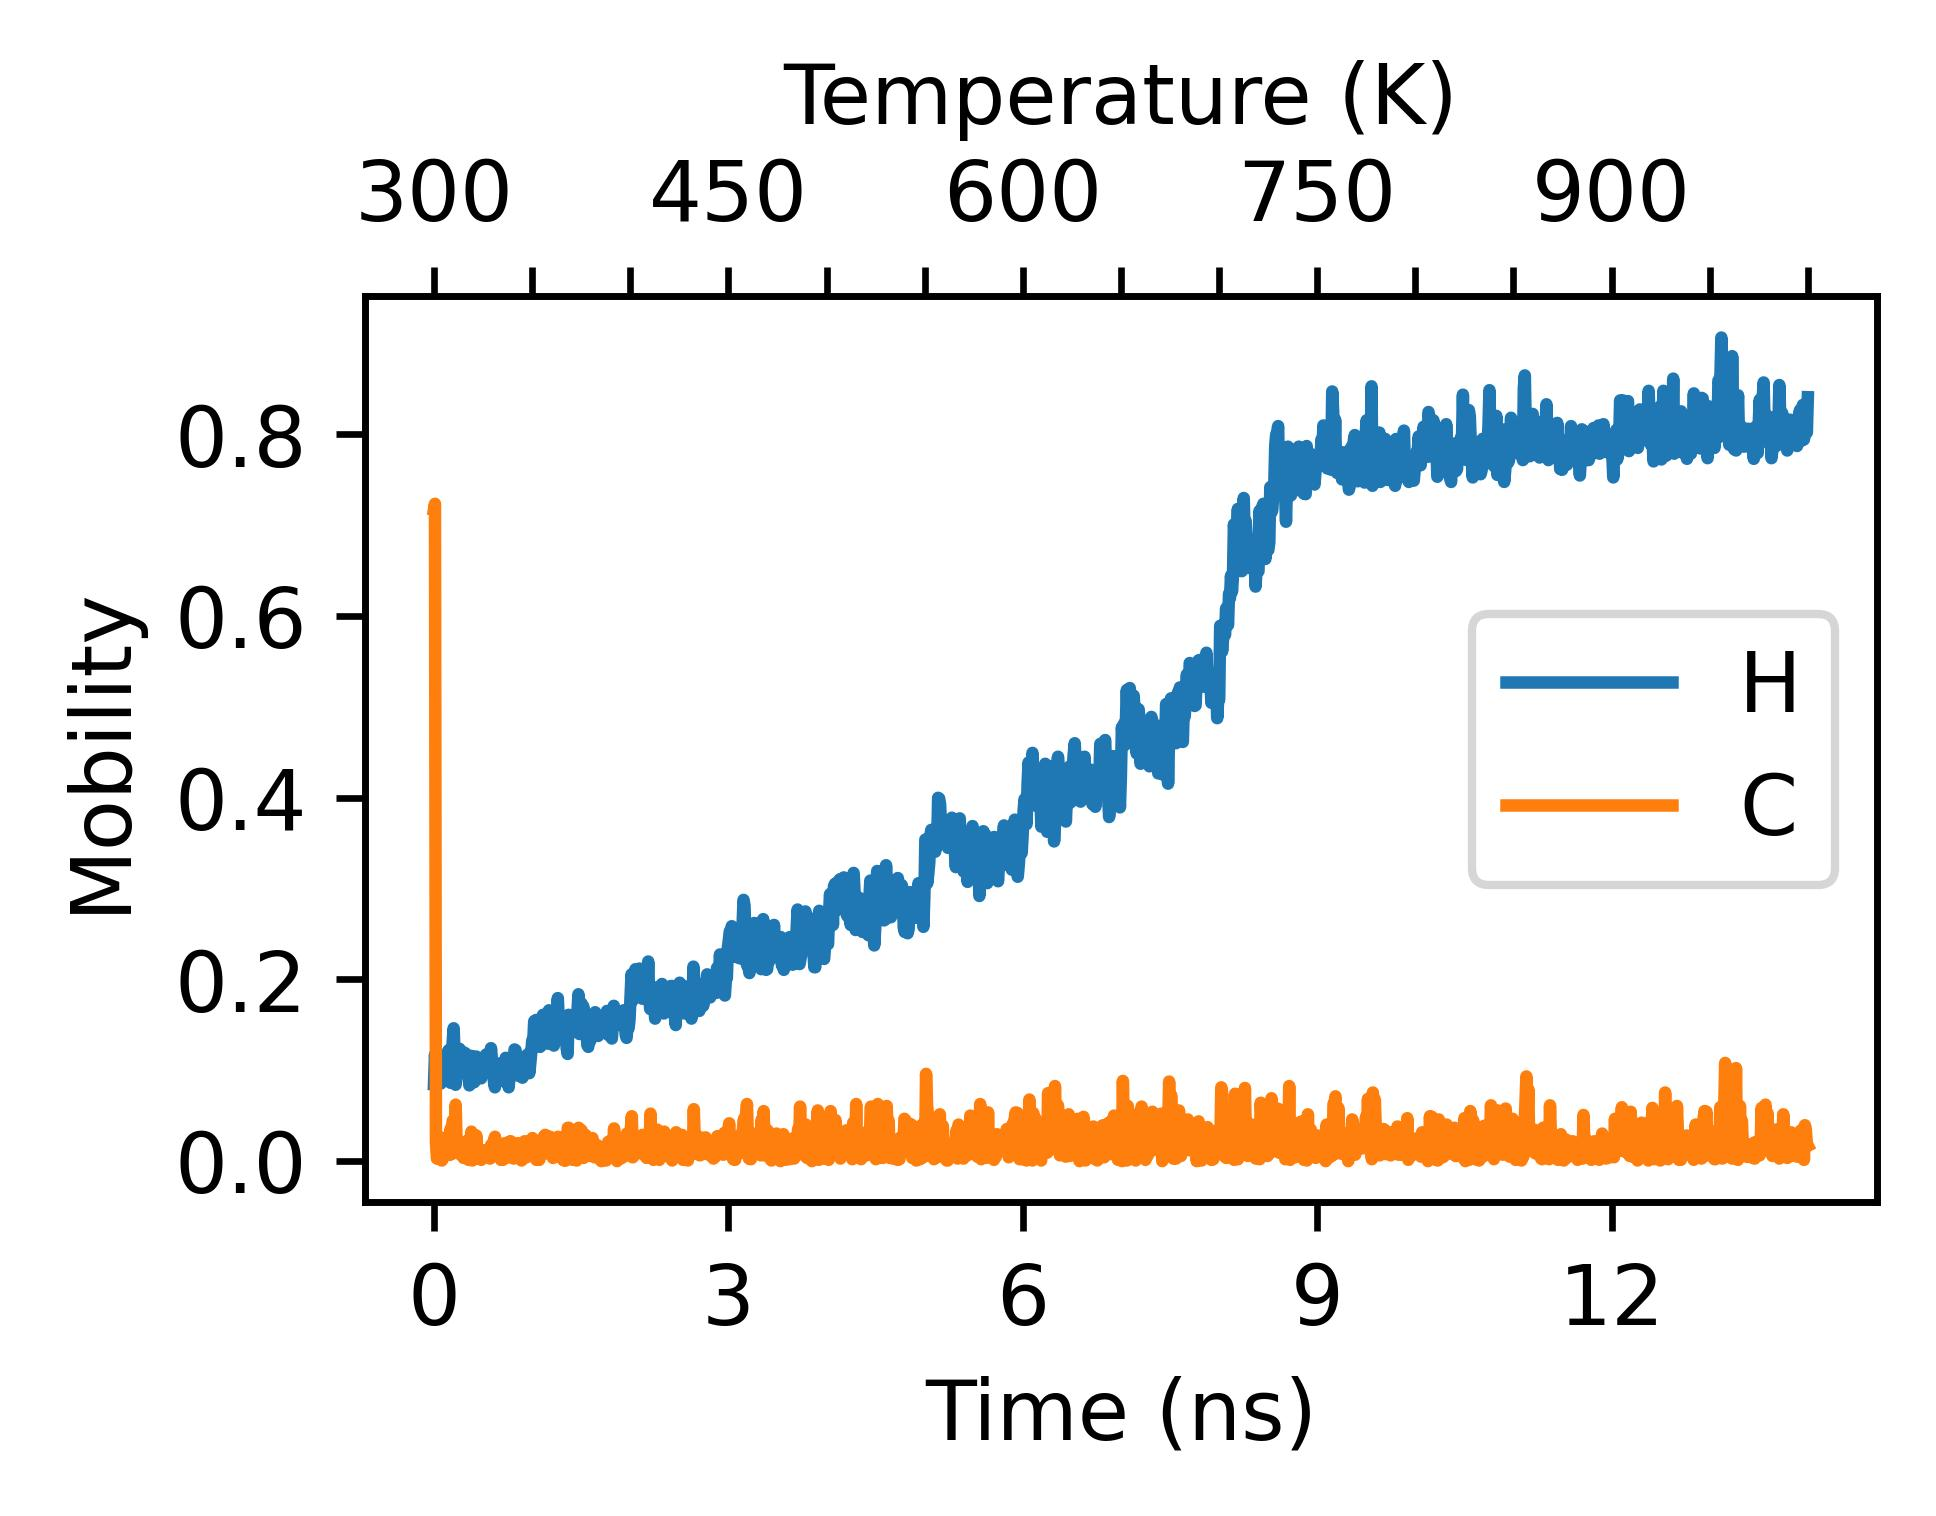
\includegraphics[width = 8cm]{figures/Sapphire/Mobility.jpeg}
    \caption{Mobility descriptors for a randomly alloyed Au$_{1149}$Pt$_{266}$ NA in the configuration of an Ih which has been rapidly heated from 300 K to 1000 K over the span of 14 ns. $\Delta t$ has been set to 10 ps.}
    \label{fig:Mobility}
\end{figure}

Single-step mechanisms involving only a section of the cluster, or multi-step processes are characterised by lower values of $C\left(t  - \Delta t, t, t + \Delta t \right)$, while continuous atomic rearrangements display C $\sim$ 0. 
This is precisely exemplified in Figure \ref{fig:Mobility}, which characterises the concertedness and collectivity of rearrangements in the AuPt NA undergoing a solid-liquid phase change when heated above 700~K.

The C statistic is consistently near 0 whilst the H statistic monotonically increases as a function of temperature. 
This is indicative of a highly dynamical object whose constituent atoms are regularly rearranging with respect to one another.
At each subsequent 10 ps window beyond 600 K, half of the atoms have a minimum of one change to their nearest-neighbour network. 
By the same token, we also draw attention to the sharp peak in the C statistic at the beginning of the dynamics. 
%
In this instance, this is representative of the collective motion of the Pt atoms within the cluster, which quickly rearrange into a more energetically favourable geometry shortly after thermal equilibration of the NA.

An intuitive and natural extension to the \texttt{Sapphire} library would be to consider the effects of ``cage breaking'' effects as presented and discussed by de Souze and Wales \cite{10.1063/1.2992128}. Such mechanisms were primarily considered from the perspective of describing diffusion in structural glass~-~formers, however, the language and order parameters presented in the article may be readily transferred to describe the nature of changes in nearest neighbours as has been presented here via $H$ and $C$. Indeed, in the reference article, the criterion for a change in atomic environment is similar to that implemented in \texttt{Sapphire}, wherein an appreciable change in the inter~-~atomic distance, as determined by the RDF, indicates a change in atomic environment. Where the real difference lies is that a cage breaking event is indicated by a minimum of two changes in the adjacency network of a specified atom. Again, reminiscent of the order parameter presented above. In the article, ``productive cage breaks'' are identified as a mechanism for driving long~-~term diffusion occurring at low temperatures. Therefore, rephrasing the analysis of diffusion events with \texttt{Sapphire} may permit the recovery of diffusion coefficients for given NAs, and provide an avenue to explore the PES in the fashion described by the authors \cite{10.1063/1.2992128}.

\subsection{Common Neighbour Analysis: signatures and patterns}
\label{sec:CNA}
%
To classify the geometrical environments of core and surface atoms, we evaluate all of the common neighbour analysis (CNA) signatures, as proposed by Honeycutt and Andersen \cite{doi:10.1021/j100303a014}, attributed to each pair of nearest-neighbour atoms. The method of determining the atomic CNA of a cluster is generalisation of the method proposed by Blaisten~-~Farojas and Andersen \cite{BLAISTENBAROJAS1985548}.

CNA signatures are of the form $(rst)$ such that $r$ is the number of nearest-neighbours common to both atoms in the pair; $s$ is the number of bonds between shared neighbours and $t$ is the longest chain which can be made from bonding s atoms if they are nearest neighbours. 
While an individual CNA signature describes the local environment of a pair of neighbours, the estimate of the percentage of how many pairs contributes to selected CNA signatures provides information on the overall nanoparticle's structure, allowing a fast classification into expected geometrical family, as icosahedral, decahedral, or FCC \cite{Baletto_2019}.
%
The main CNA signatures are (555), (422), and (421) for chemical species with a FCC bulk lattice. Although varying with the nanoparticles' size, an high concentration of (555) stands for a Ih, while FCC morphologies are expected to have 0\% of that signatures.
%
As seen for structural rearrangements, the nearest-neighbour pair can be labelled as homo- (A-A and B-B type), and hetero- (A-B) when needed. However, to describe the overall geometry of a NA, we weight in the same manner A and B atoms.
%

While proven to be successful in many cases, the CNA signature is not a property of an atom $i$.
Some commercial software, \textit{i.e.,} \texttt{Ovito} \cite{ovito}, offer a basic characterisation of each atom $i$ looking at its relative contribution to a few of known CNA signatures. Usually this criterion is able to classify only atoms in the core and when there is a clear character of each atomic environment \cite{Stukowski_2012}.
%
\texttt{Sapphire} extends the idea behind the assignment of a local crystal structure to an atom using the common neighbour analysis.

First of all, we list all the possible CNA signatures and we do limit to only a few values important in the bulk.
Per each atom, we list all the CNA signature it contributes to, and count how many times the same signature occurs (frequency chart).
The local environment of each atom-$i$ is, therefore, the collection of those signatures, and their frequency, into a CNA-pattern (CNAP). On top of the mapping following the CNAP, as highlighted in the snapshots reported in Table \ref{tab:CNA_Patterns}, we note that we can have insights on the NP-morphology on the basis of the number of different CNAPs.
%
In principle, each atom has its own CNAP, leading to have $N$ independent CNA-patterns for a nanoparticle with $N$ atoms. However, atoms in a similar environment will display the same CNAP. Therefore, the number of different CNA-patterns will decrease when the symmetry of the shape increases. Furthermore, being CNAP sensitive to the surface, and not only to core, nanoparticles limited by different facets will have more CNAPs. With this is mind, an octahedron presents five different CNA patterns while a Marks decahedron has at least 11. 
%
Table \ref{tab:CNA_Patterns} reports the CNAP distributions for common geometries classifying the most commonly observed CNAPs, and a short description of each CNAP. We do stress that no restriction to any specific signature occurs here. However, as the geometries shown are highly symmetric, overall we provide a description for a limited number of CNAPs. The CNAP is given as a string $[(\%_i,(r_is_it_i))]$, where $\%$ is the number of times the atom participates to the (rst) signature. The sum of $\%_i$ is expected to be 12 if the atom $i$ is in the core, and less for surface atoms as this sum is simply the coordination number of the atom wih that given CNAP.
%
\begin{figure}[ht!]
    \centering
    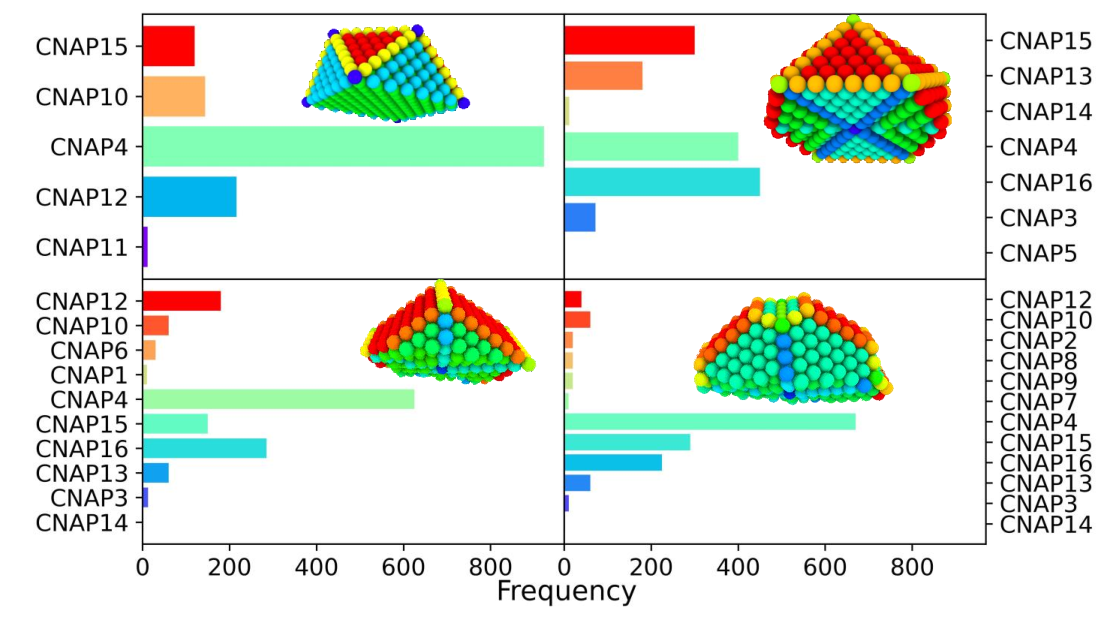
\includegraphics[width=14cm]{figures/Sapphire/CNA_Pats.pdf}
    \caption{Frequency chart of regularly-occurring CNA patterns in closed-shell geometries, namely a cubooctahedron (Co), an icosahedron (Ih), a Ino-decahedron (InoDh) with 1415 atoms, and a Marks-decahedron (mDh) with 1428 atoms. Snapshots of cut-in-half MNPs are shown in the insets, and atoms are coloured in agreement with their CNA-pattern, as listed in Table \ref{tab:CNA_Patterns}. }
    \label{fig:CNA_Patterns}
\end{figure}

\begin{sidewaystable}[ht!]
\caption{Definition of observed CNA Patterns (CNAP) and their descriptions in the common geometry in Figure\ref{fig:CNA_Patterns}. We further label when a certain CNAP can refer to atom in the core, surface, or both.}
\label{tab:CNA_Patterns}
\begin{tabular}{lc|ll}
\hline
Pattern   & CNAP-label                                                & Description & Surface 
%Found in Figure \ref{fig:CNA_Patterns} & Surface     
\\ \hline
\\[-1em]
$[(1, (100)), (2, (211)), (1, (322)), (1, (422))]$ &  CNAP1 & \makecell{Vertex from CNAP16 bordering \\ two $(111)$ facets and a $(100)$ } & Y 
\\ \hline
\\[-1em]
%
$[(1, (200)), (2, (211)), (2, (311)), (1, (421))]$   &  CNAP2   & \makecell{Edge between a $(100)$ \\ and a slightly distorted $(111)$ facet } & Y    
\\ \hline
\\[-1em]
%
$[(10, (422)), (2, (555))]$    &  CNAP3   & Atoms lying on a (555) symmetry axis & N     
\\ \hline
\\[-1em]
%
$[(12, (421))]$   &  CNAP4   & FCC bulk & N
\\ \hline
\\[-1em]
%
$[(12, (555))]$ &  CNAP5 &  Interception of six five-fold axis & N   
\\ \hline
\\[-1em]
%
$ [(2, (100)), (2, (211)), (2, (422))] $    &  CNAP6    & Edge between $(100)$ facets & Y
\\ \hline
\\[-1em]
%
$[(2, (200)), (1, (300)), (2, (311)), (1, (322)), (1, (422))]$ &  CNAP7  & \makecell{Vertex lying on twinning \\ planes shared by (111) facets} & Y
\\ \hline
\\[-1em]
%
$[(2, (200)), (4, (311)), (1, (421))]$ &  CNAP8 & \makecell{Edge between (111) re-entrances \\ and (111) facets} & Y
\\ \hline
\\[-1em]
%
$[(2, (300)), (4, (311)), (2, (421)), (2, (422))]$ &  CNAP9 & Re-entrance delimited by $(111)$ facets & Both
\\ \hline
\\[-1em]
%
$[(3, (211)), (2, (311)), (2, (421))]$    &  CNAP10  & Edge between $(100)$ and $(111)$ facets & Y
%& a.4, b.6, c.4, d.4  & Yes         
\\ \hline
%
$[(4, (211)), (1, (421))]$  &  CNAP11 & Vertex shared by $(100)$ and $(111)$ facets & Y 
\\ \hline
\\[-1em]
%
$[(4, (211)), (4, (421))]$   &  CNAP12   & $(100)$ facet  & Y        
\\ \hline
\\[-1em]
%
$[(4, (311)), (2, (322)), (2, (422))]$ &  CNAP13  & Five-fold symmetry axes (no centre) & Y
\\ \hline
%
$[(5, (322)), (1, (555))]$    &  CNAP14   & Five-fold vertex & Y
\\ \hline
\\[-1em]
%
$[(6, (311)), (3, (421))]$ &  CNAP15 & $(111)$ facet  & Y
\\     \hline
%
$[(6, (421)), (6, (422))]$ &  CNAP16 & Twinning planes  & N 
\\     \hline
\end{tabular}
\end{sidewaystable}
%

%Patterns to identify surface and bulk features are common to clusters of different shapes. 
Given the evident sensitivity to local geometry, the next question to ask is how much CNA-patterns are sensitive to imperfections in the crystalline structure and if could be used to classify a nanoparticle or nanoalloy into a certain family.
While we discussed already how we do expect the dependence of the geometrical symmetry by the number of independent CNAPs, here we would like tot stress that similar edges as the one between (100) and (111) can be identified by two patterns, namely CNAP2 and CNAP10 (see Figure \ref{fig:CNA_Patterns} and Table \ref{tab:CNA_Patterns}), depending on whether they are from a Dh or from an FCC environment. 
%
Generally speaking, an automatic classification of NAs into the distinguish three main morphology families as FCC-like, decahedra (Dh), and icosahedra (Ih), is desirable. %depending the number and type of CNA-patterns. %As pointed out in Ref.\cite{Rossi2018}, an icosahedron might show or not a centre where the five-fold axes intercept. Technically, the MNP will be a cut of an Ih or a deformed Ih, but anyway the main characteristic is to have several atoms in a non bulk-like environment.
The CNA-patterns [10,(422), 2(555)]; [4,(311), 2,(322), 2,(422)] occur in both Dh and Ih, as seen in Figure \ref{fig:CNA_Patterns}. The latter, if sufficiently symmetric, has a [12,(555)] pattern too. 
Line displacement in an FCC arrangement arise as a mixture of [(l,(422)), (k,(421))] with different l, k frequency, such as $l+k=12$.


\section{Surface Identification}

As many physical and chemical processes occur at the surface \cite{Greely2009,TRossi2020,DiPaola2016}, an automated classification of which atoms are at the surface, subsurface, and core for a given NA is welcome. 
The classification of core and subsurface atoms will be facile following a "peeling" of the outermost layer.
Core atoms are designated as those atoms that do not belong to the surface or sub-surface.
The Reader should note that combining the identification of atoms in the surface, subsurface, and core shells will permit the calculatiom of other atomistic properties, \textit{i.e.,} related to the energy when calculated as atomistic contributions.
%

While on perfectly built geometries the identification of atoms at the surface follows their coordination number, \textit{i.e.,} imposing $CN\leq 10$ to define atoms at the surface. For unknown, low-symmetry, or amorphous morphologies, this task is far from trivial.
Any classification simply based on the coordination number fails, independently of how the coordination number is calculated, as both low and high coordinated atoms can be present at the surface, see the heatmap in  Figure \ref{fig:agcn}.

A combination of a condition on $CN$ and radial distance will work only for spherical MNPs, but will fail for prolate/oblate systems. 
Hence, there is a need to find alternative approaches which require no \textit{a priori} information of the target system.
%

Amongst others, there exists a clustering approach based on local atomic environment descriptors \cite{Zeni2021}. The clustering approach was used to classify atoms in Au NPs, and implemented in the \texttt{RAFFY} Python package \cite{zeni2021compact}, and labels atoms in an unsupervised manner via hierarchical k-means clustering.
%
The atoms from one or more molecular dynamics snapshots are fingerprinted using local descriptors based on the atomic cluster expansion \cite{drautz2019} (ACE) framework. 
%
The latter encodes information of local atomic environments by approximating the local atomic density via spherical harmonics and radial basis expansions, and then constructing rotation-invariant representations from the coefficients of such expansions.
%
A cut-off radius, alongside other parameters, must be specified for the ACE descriptors; typical cut-off values are comprised between the distance of the second and third shell of neighbours.
%
This approach unbiasedly distinguishes between low-coordination surface, highly coordinated surface, and bulk atoms \cite{Zeni2021}.  
%
Moreover, it enables the discernment of locally melted and locally solid atomic environments, therefore providing a robust measure of melting and surface rearrangement temperatures.

\section{Averaging routes}
\label{sec:Ave}
There is support for creating plots for a single analysed trajectory or to consider the average over multiple, independent simulations.
%
One can toggle between these alternatives by setting the \texttt{single$\_$file} flag to be true and \texttt{iter$\_$dir} to be false, or by setting single$\_$file flag to be false and setting the \texttt{iter$\_$dir} flag to be a list of relative paths from the defined base directory to each of the iterations to be considered. 
%

It should be noted that \texttt{Sapphire} provides the arithmetic average for each of the requested quantities. Caution is advised to users who take advantage of this feature as it may not always be meaningful to compute or present such averages. 
Indeed, these meta-analyses are only meaningful if the ensemble being sampled across is consistent %expected to be approximately constant 
over time, and if the dynamics are at the equilibrium.

When reporting and presenting these ensemble averages, \texttt{Sapphire} computes uncertainties across samples as the standard error. 
That is to say that across the ensemble, we assume that all deviations are independently and identically distributed (i.i.d.). 
Indeed, the former is trivial to guarantee if multiple independent realisations of a given dynamical process have been computed.
For the extensive phase space of dynamical systems, a Boltzmann distribution is an adequate candidate for systems close to equilibrium.
However, if one is intending to probe non-equilibrium dynamics for which a steady state distribution cannot be uniquely defined at a given point in the dynamics, then the choice of distribution for describing the observables as random variables becomes more nuanced and additional care is necessary to ensure that the phase space has been adequately sampled.
%
Nonetheless, when the dynamics of the system are not far from equilibrium, this scheme provides a fast and intuitive method to visualise variance and spread in the descriptors. We have elected to present a AuPt system to demonstrate the utility of the \texttt{Sapphire} averaging scheme. 

Figure \ref{fig:ens-avg} reports four ensemble averaged quantities for a coalesced Au$_{923}^{Ih}$Pt$_{55}^{Ih}$ held at 450 K for 500 ns. Classical Molecular Dynamics simulations are done using the software package LoDiS \cite{LoDiS}.
This temperature is too low to activate structural rearrangements within the timescale sampled by the Molecular Dynamics trajectory. 
%

We define the local heterogeneous atomic environment (LAE) as being the percentage of species $B=Pt$ with $LAE$ neighbours of species $A=Au$. $LAE=0$ indicates that these atoms create no heterogeneous bonds. 
%
$1 \leq LAE \leq 6$ describes a mixed environment; while $LAE>9$ suggest that these atoms (Pt) are almost totally encapsulation by species $Au$ atoms.
%
Initially, we note that all descriptors are found to have only small inter-sample variations at approximately 10\% of the mean value. 
All the descriptors considered, namely the radius of gyration (RoG), the number of Pt at the surface (Pt$_{surf}$, LAE of Pt, and the distance between the sub-region centres of mass $\Delta(CoM)$, versus time, show that a structural transformation occurs at the beginning (below 100 ns), with Pt incorporating inside the Au core and decreasing the number of Pt at the surface. At the same time, we do recognise other two steps.
The small plateaux between 100-200 ns where $\Delta(CoM)$ is almost flat indicates a small changes in the LAE has occurred. After 200 ns, we observe a increment in the Pt mobility and a change of the chemical distribution of Pt atoms in the NA.

\begin{figure}[ht!]
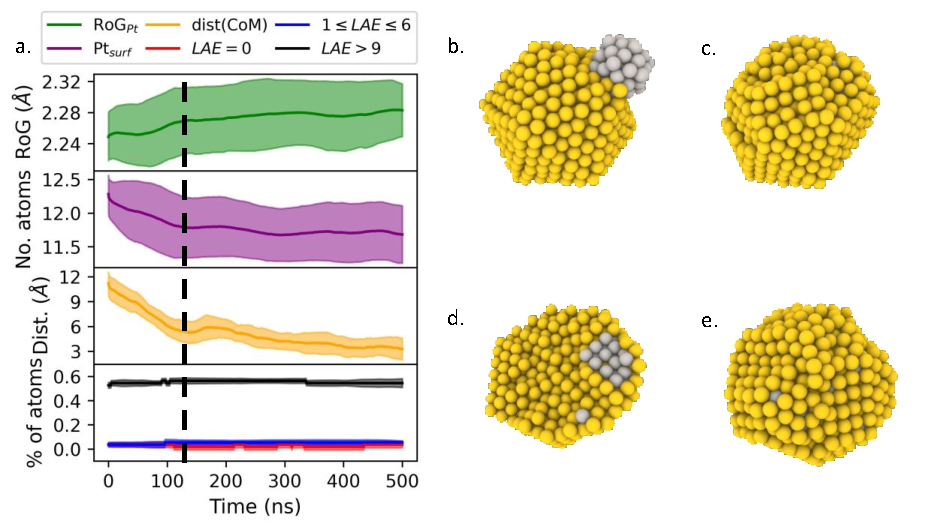
\includegraphics[width=16cm]{figures/Sapphire/Sapphir_Avg.pdf}
\caption{\textbf{a.} Ensemble averaged evolution of atomic descriptors for a coalesced system of Au$_{923}^{Ih}$Pt$_{55}^{Ih}$ thermalised at 600 K for 500 ns. From top to bottom, the radius of gyration of the Pt sub-region only; the number of Pt atoms at the surface, based on the definition from the CNAP; the $\Delta(CoM)$ between the centre of mass of the two sub-regions, and the LAE of Pt atoms. Subsequent panels depict the atomic configuration at \textbf{b.} the initial deposited stage, \textbf{c, d.} $125$ ns at the point identified by the dashed line in panel \textbf{a.}. \textbf{c.} Is the full structure, and \textbf{d.} is a cross section to show the Pt distribution within the cluster. \textbf{e.} }
\label{fig:ens-avg}
\end{figure}
We do not present these averaging techniques to serve as a replacement for an individual's choice of averaging routine, as these are unique and particular to the dynamics and quantities under consideration. Rather, we present this utility as a means to explore and present variations across i.i.d. samples.

\section{Structure - Properties relationships}

The \texttt{Sapphire} library focuses on the characterisation of MNPs and NAs morphology.
%and to provide structural insights.
%
Nonetheless, \texttt{Sapphire} can be used in synergy with available codes geared toward the prediction of chemophysical properties of MNPs and NAs.
%
In the next sub-sections we briefly discuss three examples, where:
\begin{itemize}
    \item \texttt{Sapphire} leverages ASE to move back to energy-related properties; 
    \item \texttt{Sapphire} exploits a link with a microkinetic model \cite{Gazzarrini2021} to estimate the activity over certain reduction reactions; \item \texttt{Sapphire} is connected with the pyGDM \cite{GDM} library to qualitatively estimate the optical properties, absorption and extinction spectra, of mono- and bimetallic nanoparticles.
\end{itemize}

\subsection{From structure to energy} 
Often it is desirable to check the energy stability of a certain shape or chemical ordering. 
Currently, ASE supports effective medium (EMT), the embedded atom method (EAM), and the \texttt{kimpy} calculators. EAM benefits from the Interatomic Potentials Repository Project available at \url{https://www.ctcms.nist.gov/potentials/}, while OpenKIM is a recent NSF project devoted to provide access to  classical interatomic potentials. Unfortunately, SMATB calculators are not currently available. They were part of the ASAP3 distribution \cite{asap3}, which has since been deprecated and discontinued.
In the manual and tutorials we demonstrate how \texttt{Sapphire} may interface with ASE and its library of calculators to compute energetics. Given the broad support for potential calculators in the ASE distribution, one is at liberty to select their own theory of choice for their particular system.

\subsection{Electrocatalytic properties via a microkinetic model}
\label{sec:electrocat}

As has been demonstrated and discussed in the literature \cite{https://doi.org/10.1002/cphc.201900564,C9NA00252A}, the aGCN as defined in Equation \ref{eqn:aGCN} can be employed as geometrical descriptor for both oxygen and CO$_{2}$ electrochemical reduction \cite{C6SC04788B,doi:10.1021/acscatal.7b01194}. At an applied potential $U$, and temperature
$T$, an isomer characterised by a specific aGCN fingerprint 
produces a current density from a reaction step associated with
a free~-~reaction energy $\Delta G$, given by a simple micro-kinetic model, j$_{\mathrm{nanoparticle}}$(t,T,U). For such an electro-chemical process, the full expression can be written as:
\begin{eqnarray}
j_{\mathrm{nanoparticle}}(t,T,U) &=&\sum_{\alpha} \mathcal{C} \xi(t,T)\alpha
e^{\beta \Delta G (U, T, \alpha)} \mbox{~,}
\label{Eq:jnp}
\end{eqnarray}
where $\Delta G (U, T, \alpha)$ labels the reaction free energy at the applied potential $U$ and temperature $T$, which is also a function of the descriptor $\alpha$, $\beta$ is the Maxwell-Boltzmann factor, $\xi(t,T) = \frac{\Omega(\alpha)}{N_{\mathrm{site}}(t,T)}$ is the fraction of non-equivalent adsorption sites $\Omega(\alpha)$ to the total number of sites available, $N_{\mathrm{site}}$, the prefactor $\mathcal{C}$ is fitted to reproduce the known specific current of low-Miller-index surfaces, and the sum runs over the collection of the non equivalent sites appearing in the nanoparticle under consideration. The latter are also being categorised by their $\alpha$ values. Indeed, a similar model was proposed and deployed by Tripkovic \textit{et al} in which $\Delta G$ was computed within a DFT framework for adsorption sites on low Miller~-~Index surfaces \cite{Tripkovic2014-wl} .
%
%Note that, for a fixed overpotential U, temperature T, and nanoparticle geometry, the specific activity of a nanoparticle is determined solely by the scaling relationship between $\Delta G$ and the $\alpha$ descriptor of choice, and number and kind of non equivalent adsorption sites at the nanoparticle surface.
    %
Note that in \ref{Eq:jnp} the effect of the potential is treated as an \textit{a posteriori} correction, in line with the computational hydrogen electrode model \cite{Norskov1998}. 
%
The aGCN, Equation \ref{eqn:aGCN}, of a surface site is an accurate descriptor to predict the activity of a metallic adsorption site, as demonstrated for Au, Cu, Pt, PtNi, catalysing the electrochemical reduction of oxygen or carbon dioxide  \cite{Calle-Vallejo2014,Calle2015,Zhao2016}.
%
Assuming a volcano-plot relationship, 
the reaction free energy $\Delta G$ and the aGCN are related by the following general expression:
\begin{equation}
\Delta G =
    \begin{cases}
     + a1 ~ \textrm{aGCN}_n - b1 ~~~~\textrm{if~ aGCN}_n<~ aGCN^{volcano-peak} \\
     - a2 ~ \textrm{aGCN}_n + b2 ~~~~\textrm{if~ aGCN}_n> aGCN^{volcano-peak} \\
    \end{cases}
    \mbox{~~~.}
\label{eq:volcano}
\end{equation}
%
where the coefficients a1, b1, a2, b2, and the value of the $aGCN^{volcano-peak}$ should be derived from a small set of DFT calculations, if not available in the literature \cite{FCVChemSci2018}. For example, the case of the oxygen reduction reaction on Pt nanoparticles \cite{Rossi2020}. Whilst the determination of a current density via this protocol has not yet been explicitly computed via \texttt{Sapphire}, the precise formulation provided by Rossi \textit{et al} \cite{Rossi2020}, and implemented by Gazzarrini \textit{et al} \cite{Gazzarrini2021} have been adopted within \texttt{Sapphire}.

Once the Gibbs free energy is defined in terms of the aGCN, a quantity that can be monitored during the lifetime of a MNP, we can establish relationships between the ageing of a MNP, referring to its structural stability, and its activity. Examples have been reported previously by our group for ORR on Pt \cite{Rossi2020}, and for the conversion of CO$_{2}$ into methane on Cu NPs \cite{Gazzarrini2021}. Under the assumption of identifying robust structure-activity relationships, we do not see any limitation in using the scheme for NAs and for other chemical reactions.

\subsection{Optical properties via semi-classical methods}

For a fast evaluation and screening of the extinction spectrum of nanoalloy, one can adopt a classical approach, via the Green's Dyadic Method (GDM), \cite{GDM,Girard_2005} as implemented in the pyGDM code \cite{pyGDM,pyGDMarXiv}.
%
At its core, this library constructs a refractive environment via the construction of a 3D mesh of dipole oscillators whose physics is predicted within the quasi-static coupled dipole approximation.
%
It then uses an efficient and generalised propagator to predict the extinction spectrum associated to the user-defined mesh. For example, this mesh may be defined from a series of coordinates consisting of multiple constitutive components. 
%

To evaluate the extinction spectrum,  we need only to consider the interaction of the dipole moment and total field in each discretised volume cell and we proceed to employ equation \ref{eqn:ext_gdm} in the precise fashion discussed in Sec. \ref{sec:GDM} .

All metallic dielectric parameters used in these calculations are provided by either experimental work \cite{PhysRevB.6.4370,Rakic:98,PhysRevB.15.4115}, or from \textit{ab initio} investigations \cite{doi:10.1063/1.3243762}.
%
The interested reader is referred to previous literature for further detail \cite{GDM,pyGDM,pyGDMarXiv}.
%

\begin{figure}[ht!]
    \centering
    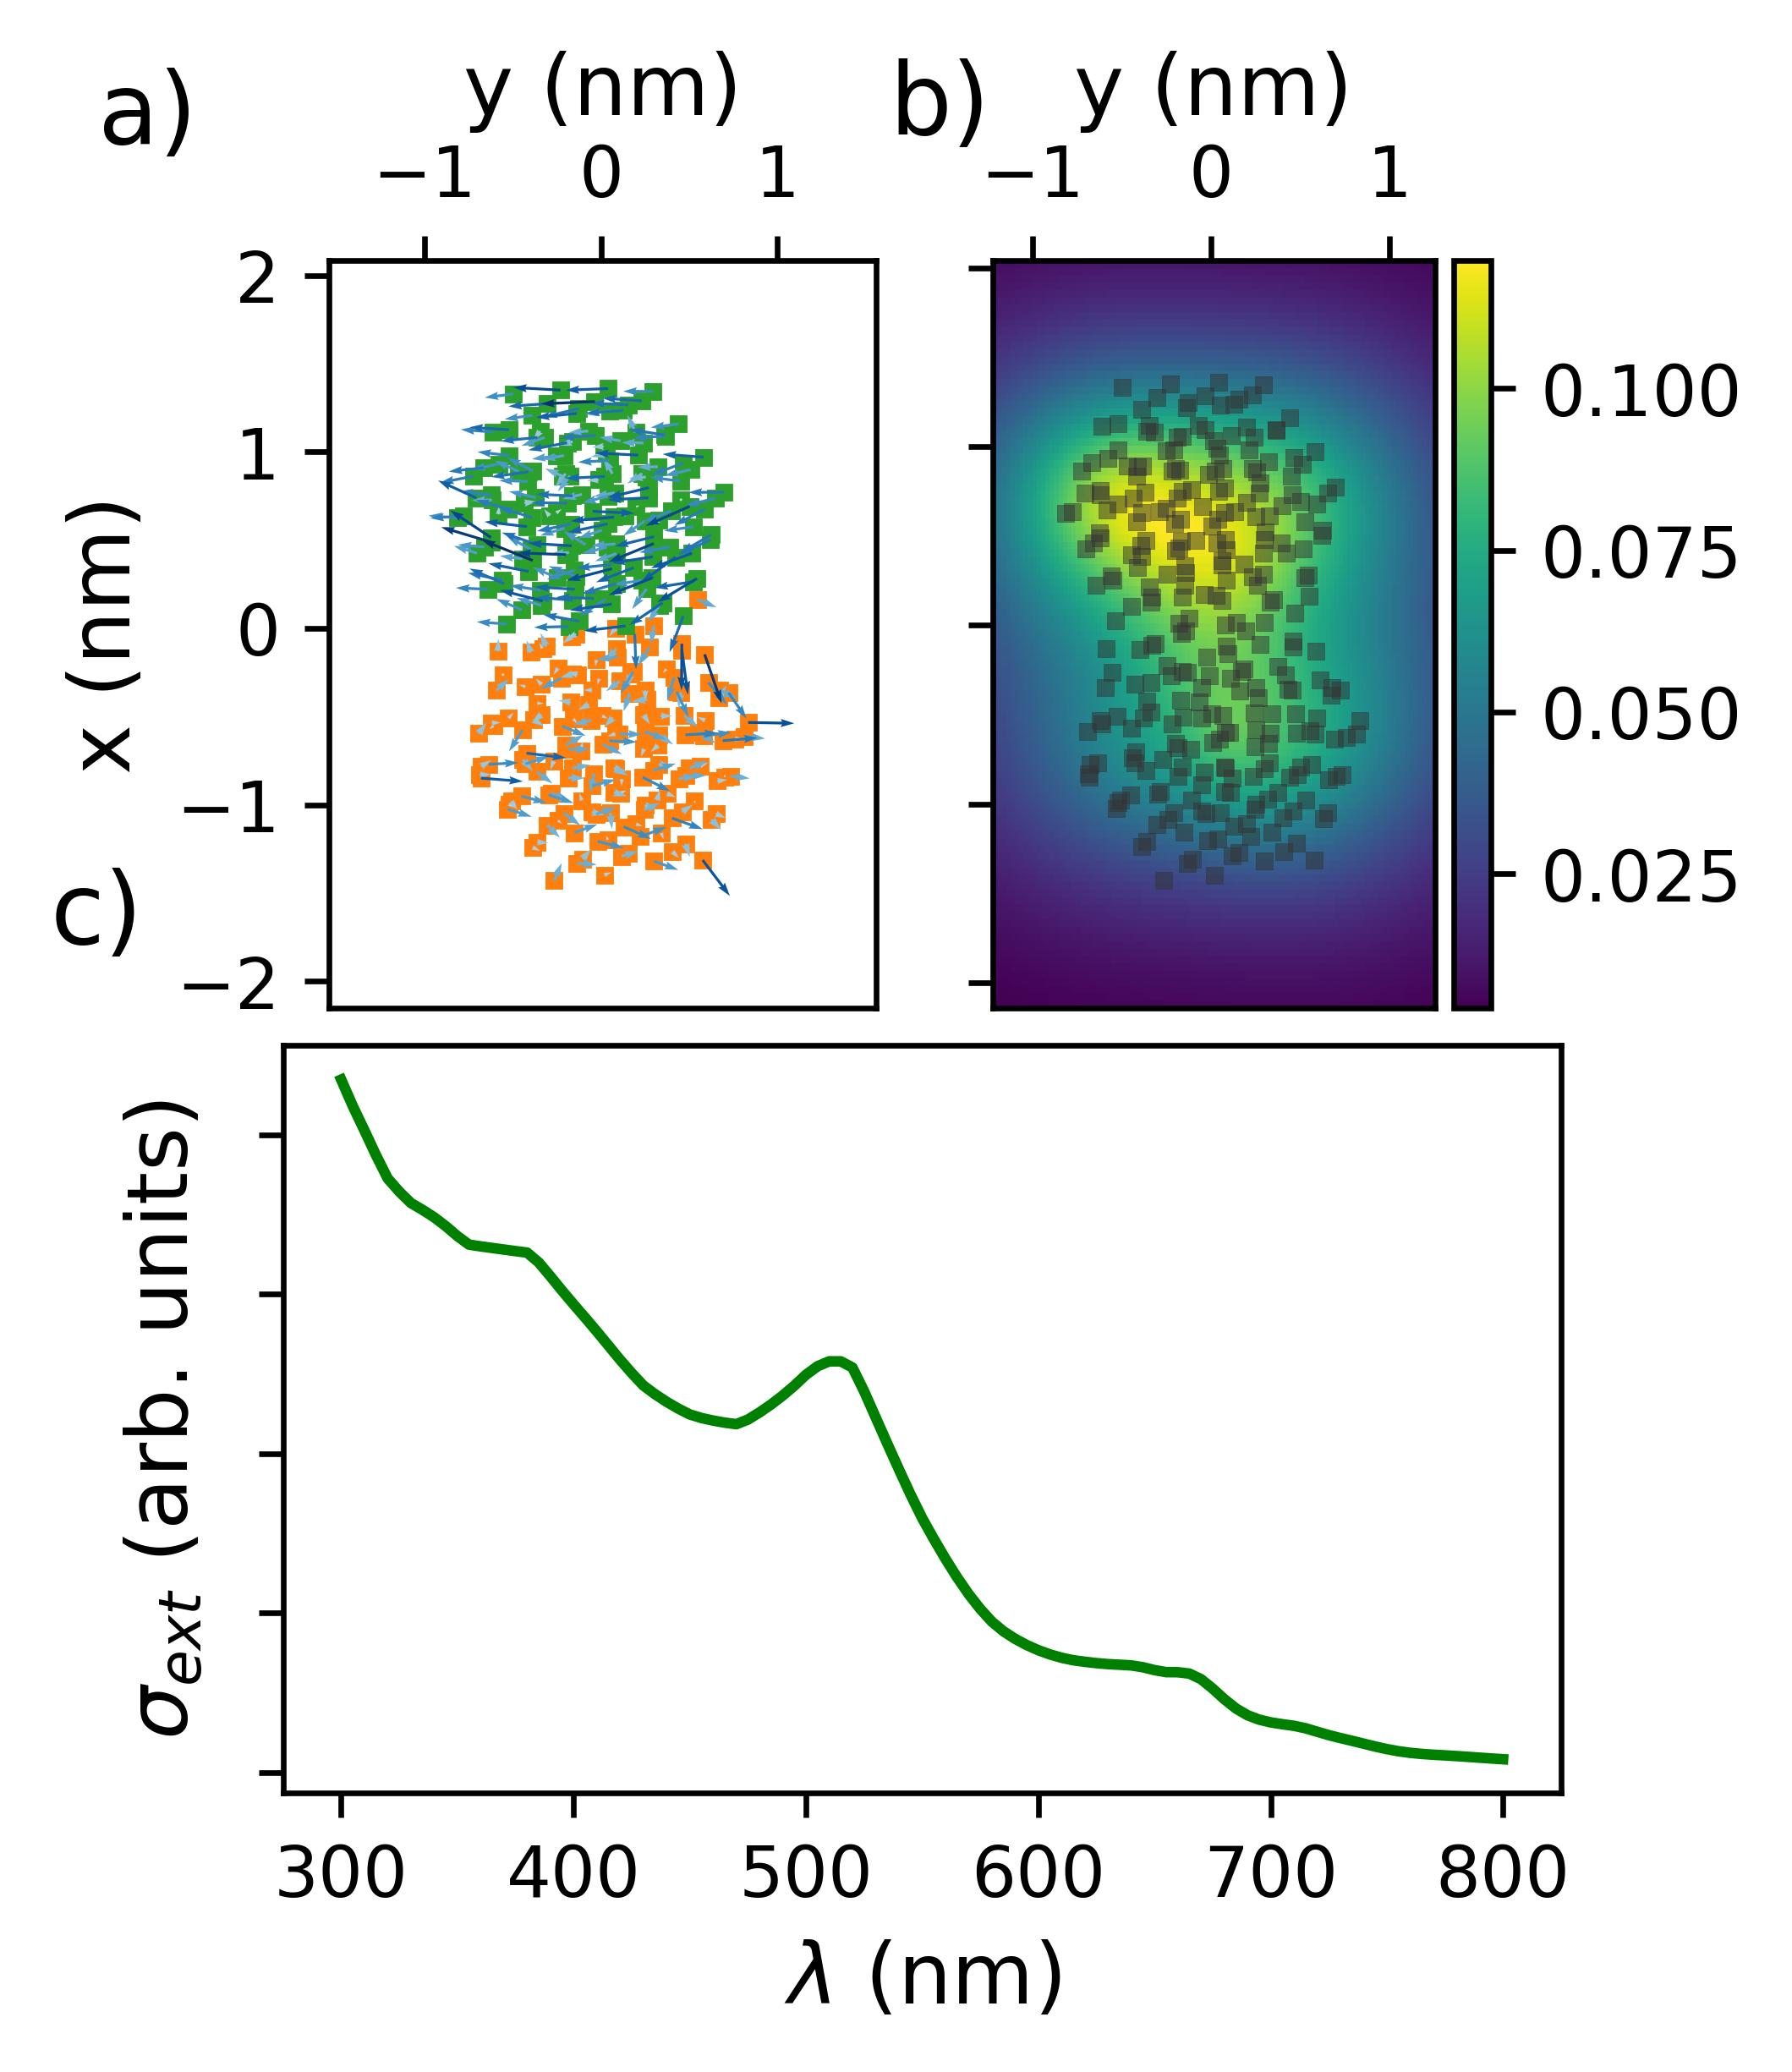
\includegraphics[width=8cm]{figures/Sapphire/Faraday_Light.jpeg}
    \caption{An illustration of the interaction between \texttt{Sapphire} and \texttt{pyGDM}. Top left, Au$_{1132}^{Ih}$Pt$_{283}^{Ih}$ consisting of Au (orange), and Pt (green) showing a Janus chemical ordering. Top-right, the local field intensity under 520 nm illumination. Bottom panel, the computed extinction spectrum for the NA}
    \label{fig:light}
\end{figure}

Any behaviour that may arise from quantum many-body effects is neglected.
Furthermore, when considering structures with size $\sim$ 1 nm illuminated in the UV~-~Vis~-~NIR, the incident field will only weakly couple to the structure. 
This results in non-trivial internal field enhancement.

Figure \ref{fig:light} reports the dipole mesh reconstructed from atomic coordinates and species in the left set of panels, and the near-field enhancement at 520 nm plane wave illumination on the right side. Intensity, as described by the colour bar, is reported as $|\mathbf{E}\left(\mathbf{r}\right)|^{2}/|\mathbf{E}_{0}|^{2}$, the strength of the field relative to the amplitude of the illuminating wave.
In the bottom panel, we present the extinction spectra computed via Equation \ref{eqn:ext_gdm} for four each of the different systems taken in consideration.
%
We have elected to present these systems to demonstrate the utility in being able to directly map a set of atomic coordinates, as may be parsed from a structural file, to a mesh of coupled dipoles with pre-defined dielectric properties. 

\section{Discussion}
The characterisation and classification of the morphology and chemical ordering in mono-, bi-, and multi-metallic NAs is a key ingredient towards rationalising their chemo-physical properties.
%

The necessity of an open-source robust, reproducible, and FAIR compliant post-processing tools, which caters the needs of the NA computational modelling community, is more and more evident.
\texttt{Sapphire} is tailored specifically to address this need by providing a library of standardised analysis tools for NA characterisation.
\texttt{Sapphire} is indeed an open-source, modular, user-friendly platform to characterise a nanoparticle's  architecture observed during, \textit{e.g.,} atom coordinates reconstructions from experiment,
molecular dynamics, or Monte Carlo based sampling.

Within \texttt{Sapphire}, several order-parameters and descriptors can be calculated, namely: pair distance and radial distribution functions, 
inertia tensors and quantity derived from the latter, coordination distributions and other topological descriptors (generalised coordination and common neighbour analysis) derived from adjacency matrices. 
\texttt{Sapphire} also provides tools for detailed analysis of the surface of NAs.

 A salient point which we have not yet addressed is that of timescales. We have presented in the work of \texttt{Sapphire} dynamical simulations on the order of nanoseconds in length. As has been discussed in the previous chapter, it is not uncommon for reconstruction events observed in the context of NAs to occur on the order of minutes to hours. We have already argued that such times are beyond reach at this level of theory, which therefore invites the question of how may we adequately sample the PES of candidate structures with \texttt{Sapphire}. A clear, and natural answer, is to incorporate methods described in Section \ref{sec:md_opt}. Among these would be methods such as basin hopping, and the iterations thereof discussed earlier, as this is an efficient method for determining the equilibrium geometry of an NA and map out local minima existing on its PES.

In the long term, it is our vision that \texttt{Sapphire} may serve to create a standardised, meaningful, characterisation and classification tool for nanoalloys. 
This will be the first critical stage in creating a comprehensive community database for such complex systems.
